In this chapter of the book we will have a closer look
at different sourdough starter types and their respective
traits.

\begin{table}[htp!]
    \begin{center}
        \documentclass[tikz]{standalone}
\usepackage{tikz}
\usepackage{siunitx}
\DeclareSIUnit\degF{\text{°}F}

\begin{document}
\begin{tabular}{|l|l|l|r|l|}
\hline
\textbf{Starter type} & \textbf{Hydration in \%} & \textbf{Flour type}     & \multicolumn{1}{l|}{\textbf{Yeast activity}} & \textbf{Bacterial activity} \\ \hline
Regular               & 100                      & Strong wheat flour      & Balanced                                     & Balanced                    \\ \hline
Liquid                & 500                      & Very strong wheat flour & Minimal                                      & High                        \\ \hline
Stiff                 & 50-60                    & All wheat flour         & High                                         & Low                         \\ \hline
\end{tabular}
\end{document}

        \caption{A comparison of different sourdough starter types and their
            respective properties. The only difference is the level of water (hydration)
        that is used when feeding the starter.}%
        \label{tab:starter-types-comparison}
    \end{center}
\end{table}

Depending on the flour you have at hand, the type of starter changes. With more
bacterial activity you have more gluten consumption of your microbes. So if
you want to bake a free standing loaf, you need a flour with more gluten. The
more gluten you have, the more of it can be broken down whilst still maintaining
dough integrity. If you live in a country where the climate to grow wheat
isn't ideal and you only have weaker flours, then a stiff sourdough starter
could be advised. The stiff sourdough starter will improve yeast activity and
reduce bacterial activity. If you are a chaser of a very sour bread and have a
very strong wheat flour then you can try to play with a liquid sourdough
starter. The key difference between all of the starters is how much water
is used in the starter. The regular starter has a 1:1 relationship of flour
to water. The liquid starter has a 5:1 water-to-flour ratio, and the stiff
starter has half the flour as water.

\begin{figure}[!htb]
\begin{center}
  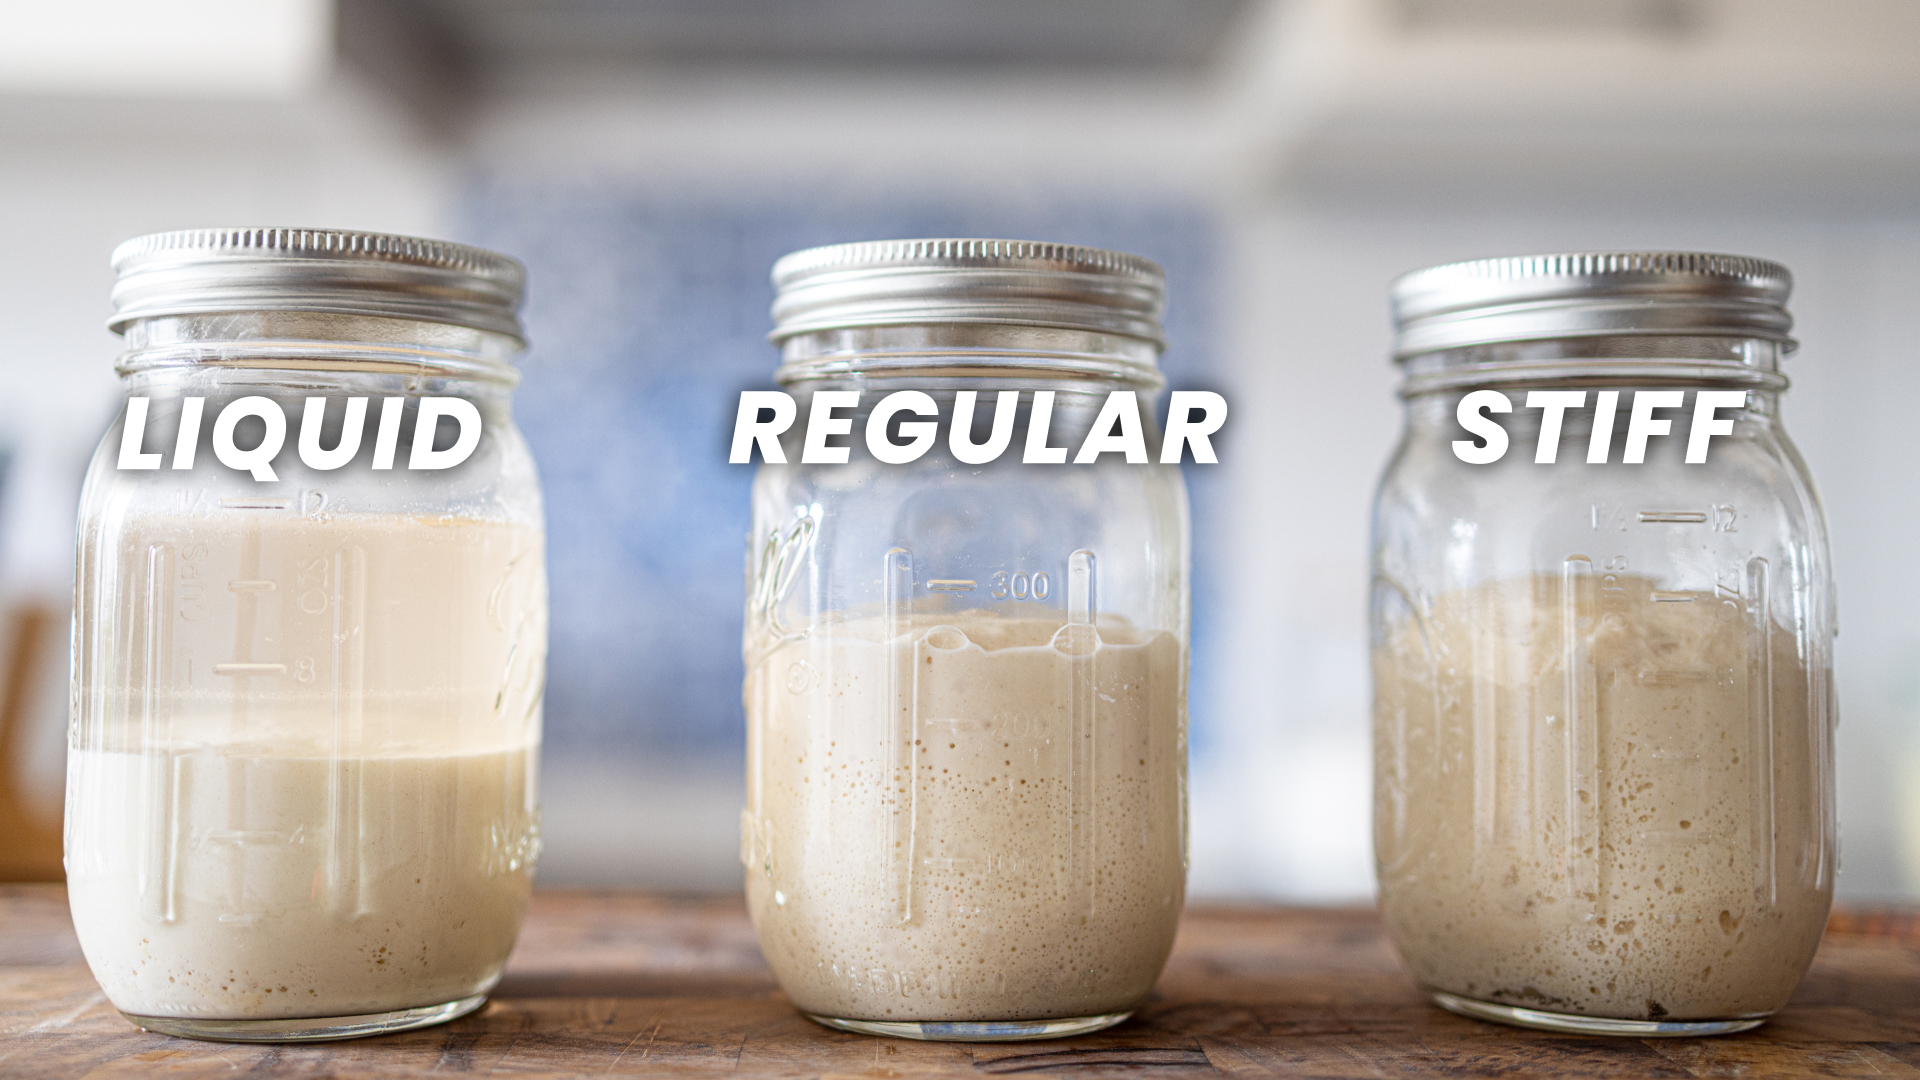
\includegraphics[width=\textwidth]{sourdough-starter-types}
  \caption{3 different starter types next to each other. Note how the liquid starter is submerged
  in water. It has a hydration of 500 percent or more.
  The regular starter has a hydration of around 100 percent, the stiff starter
around 50 to 60 percent.}%
  \label{fig:starter-types}
\end{figure}


You can change your starter type by just adjusting the feeding ratio of how
much flour and water you use. I~frequently change my starter type from
regular to liquid and then back to a stiff starter. After changing the
environment of your microbes, apply feedings at the same ratio over a couple of
days so that they can adapt to the new environment. I~typically see
changes after a single feeding, but I~recommend 2 to 3 feedings, one feeding per
day, to see a stronger effect.

Your dough is generally just a big sourdough starter. So your starter is going
to adapt and regrow inside of your main dough. But you can influence the
properties that your starter carries over to your main dough. If you have more
bacterial fermentation, then your dough will also have slightly more bacterial
fermentation. If you have more yeast fermentation, then your main dough will
have slightly more yeast fermentation. This is important to know when you are
working with a more mature unfed starter. Let's say your starter had last been
fed 48 hours ago. Chances are that your bacteria is very active while the
yeast could be dormant. In such a case you can skip feeding your starter
before making another dough. Just use a very tiny amount of starter. For 1000 g
of flour I~would take around 10 g of starter (1 percent in terms of baker's
math). If my starter is very young and had just been fed 6 to 8 hours ago I~might
end up going up to 20 percent of starter. Remember that your dough is nothing
else other than a big starter. It will tremendously help you to figure out
your best next steps.

When using such a low inoculation rate (1 percent), you need to use stronger
flour when making wheat-based doughs. Your flour naturally breaks down due
to enzymatic activity. It might take 24 hours for the starter to re-grow
inside of your bread dough. At the same time, the enzymatic activity might
have caused your gluten to degrade significantly. While this is okay
when looking at your starter, your wheat-based dough will flatten
out during baking and no longer have the typical characteristics (fluffy crumb
structure). A stronger flour with more gluten is thus advised. It allows for
a longer fermentation before most gluten is broken down.

\section{Regular starter}

\begin{figure}[!htb]
  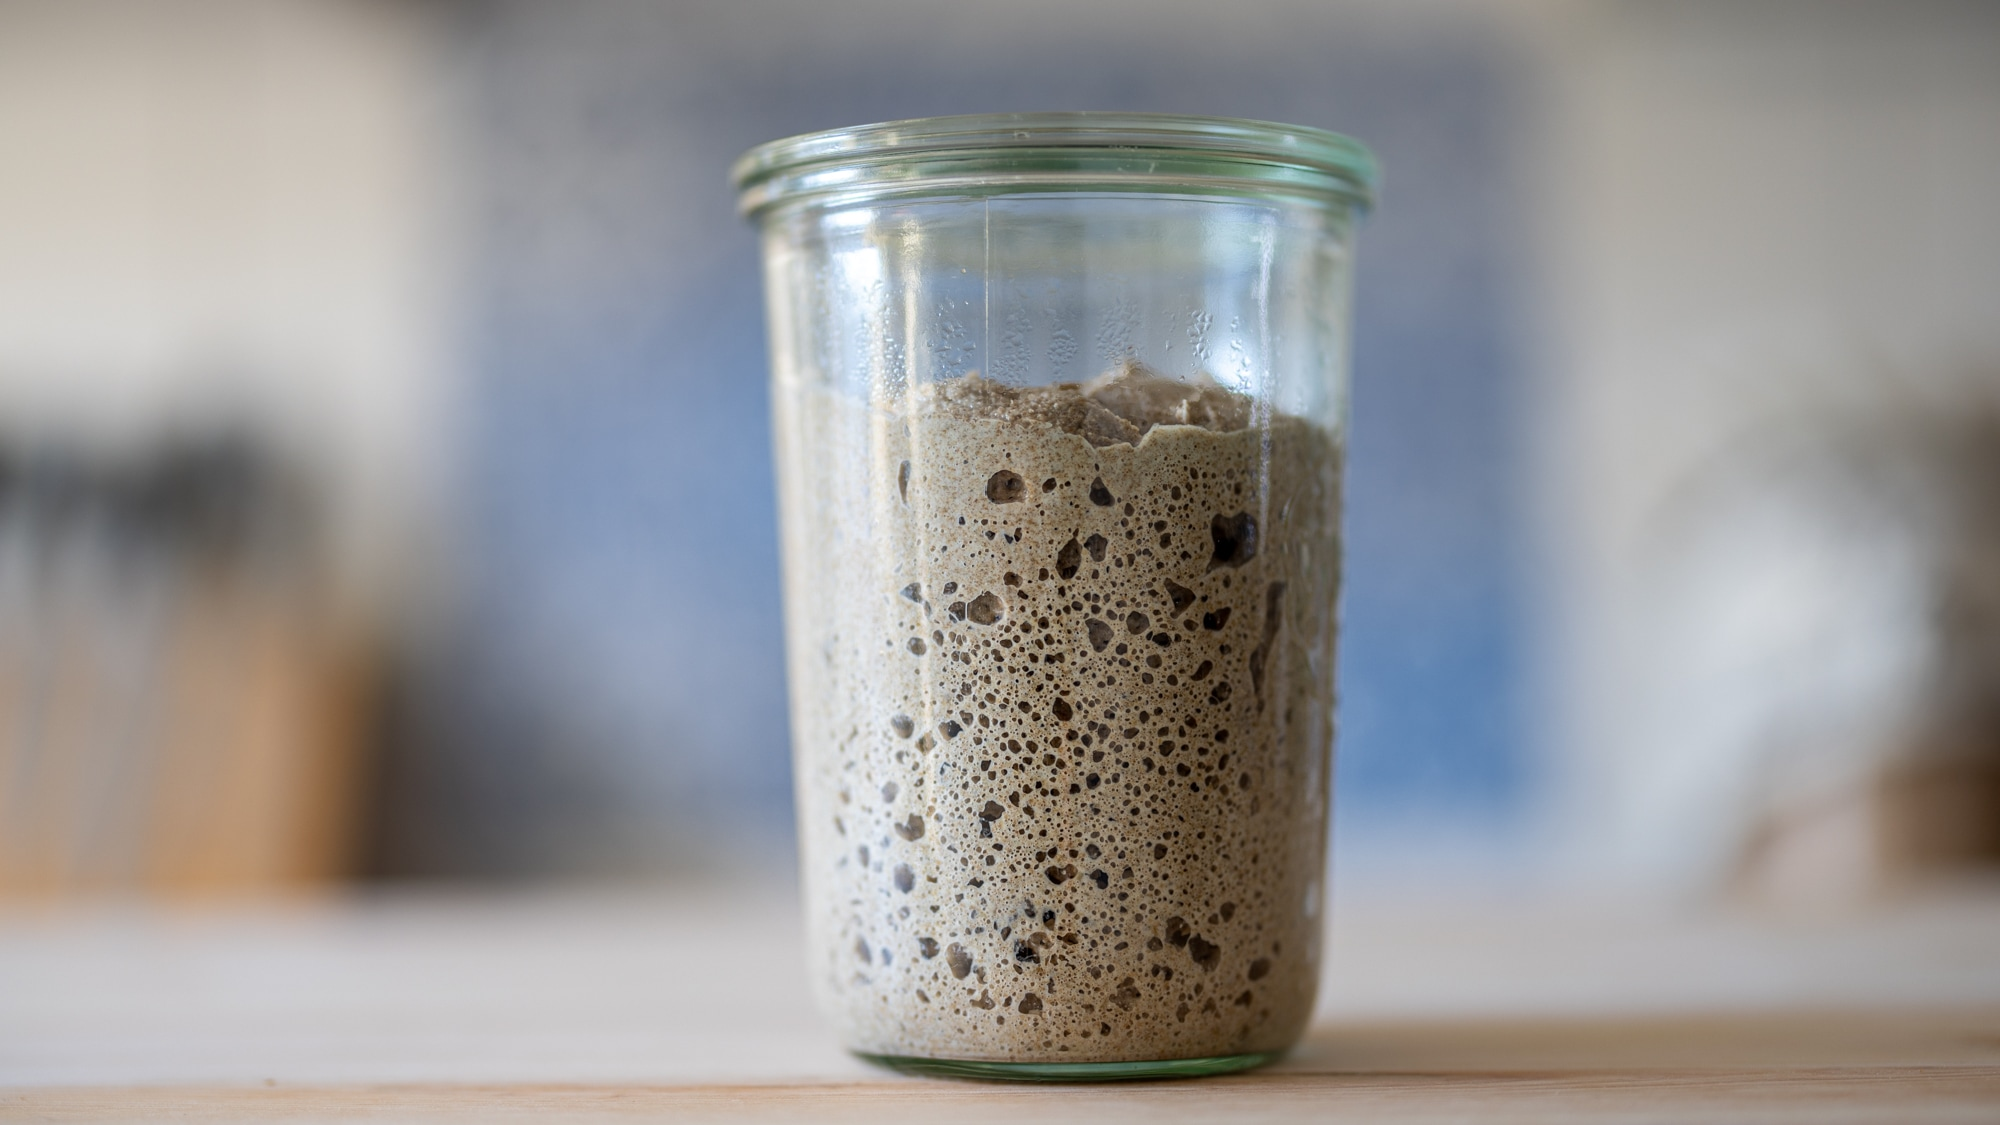
\includegraphics[width=\textwidth]{sourdough-starter.jpg}
  \caption{A regular sourdough starter at 100 percent hydration fed with rye
  flour.}%
  \label{fig:regular-sourdough-starter}
\end{figure}

The regular sourdough starter is made at a hydration of around 100 percent.
This means the starter has equal parts of flour and water. This is the most
common and most universal sourdough starter there is. The starter has a good
balance of yeast and bacteria. After a feeding, the volume increases and
increases. After it reaches a certain peak, it will start to collapse again.

The best way to judge whether the starter is ready is to look at signs such as
air pockets on the edges of your container. Also use the nose to evaluate the
smell of your starter. If you feel that the starter doesn't perform in a
desirable way, chances are that your yeast and bacteria ratios are off. In that
case frequent daily feedings using a 1:5:5 (starter:flour:water) ratio will
help.

A regular starter is a perfect choice to use when utilizing stronger wheat or spelt flours.
It also nicely works with rye, emmer or einkorn. If you only have a weak flour
at hand with less gluten, this starter might cause issues. As you tend to have
quite some bacterial activity, gluten is going to be broken down fast. When
using the starter, use around 1 to 20 percent starter based on the flour of your
dough.

Depending on the bacteria cultivated, a regular starter either has a lactic (dairy),
a vinegary (acetic) or mix of both flavor profiles. You can adjust your
starter's flavor by changing the type to a liquid starter.

\section{Liquid starter}%
\label{section:liquid-starter}

\begin{figure}[!htb]
\begin{center}
  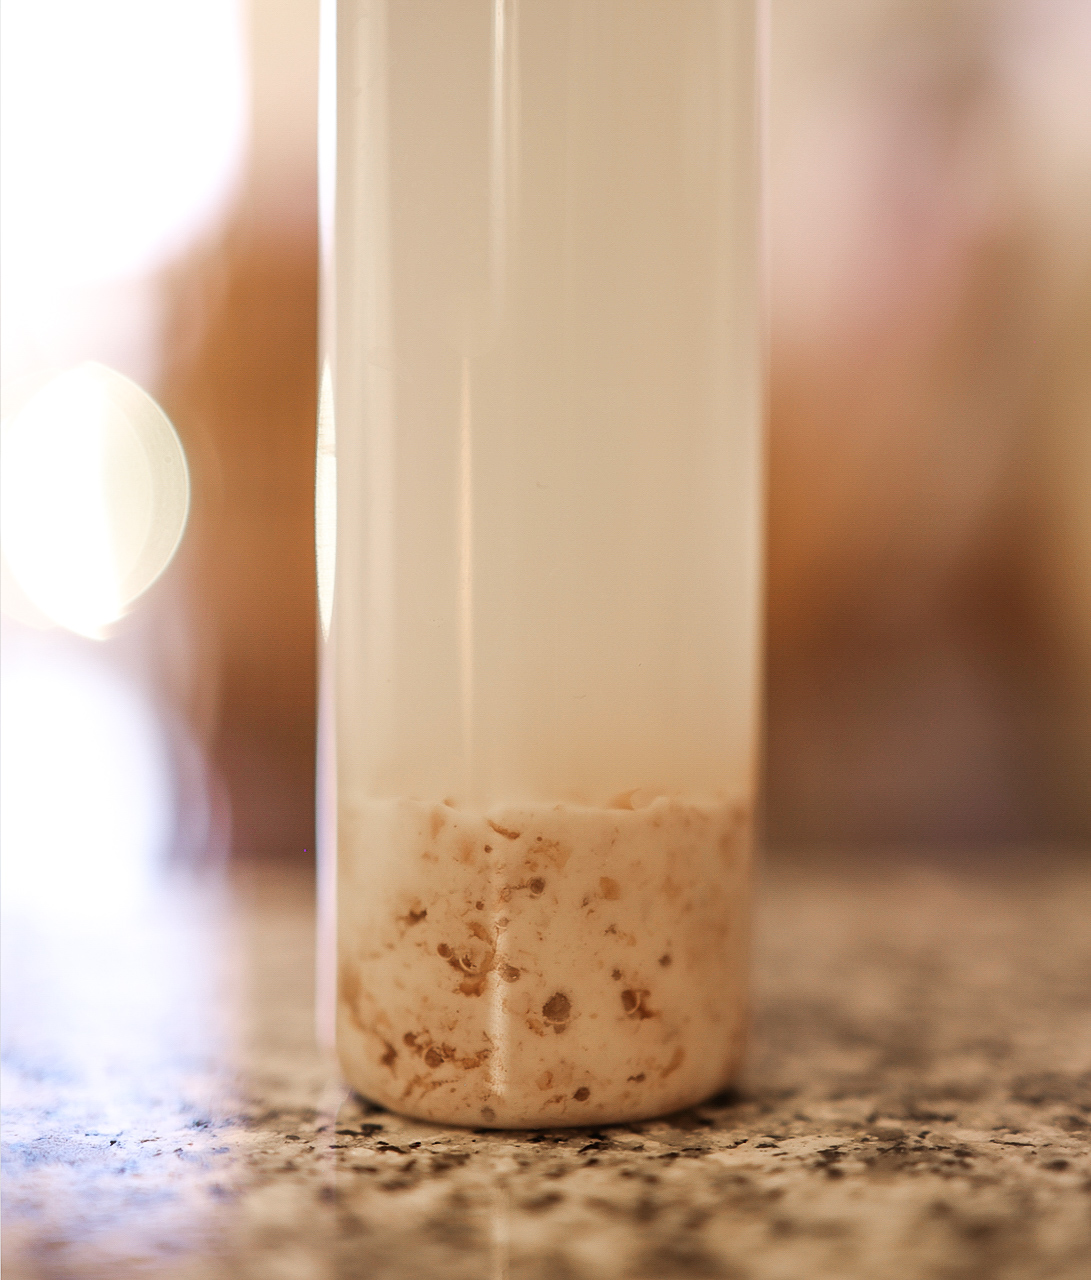
\includegraphics[width=0.5\textwidth]{sourdough-starter-liquid.jpg}
  \caption{A liquid sourdough starter features a high level of water. The high
  water amount boosts lactic acid producing bacteria. After a while the liquid
  and flour start to separate. Bubbles on the side of the flour
  indicate that the starter is ready to be used.}%
  \label{fig:liquid-sourdough-starter}
\end{center}
\end{figure}


\begin{figure}[!htb]
    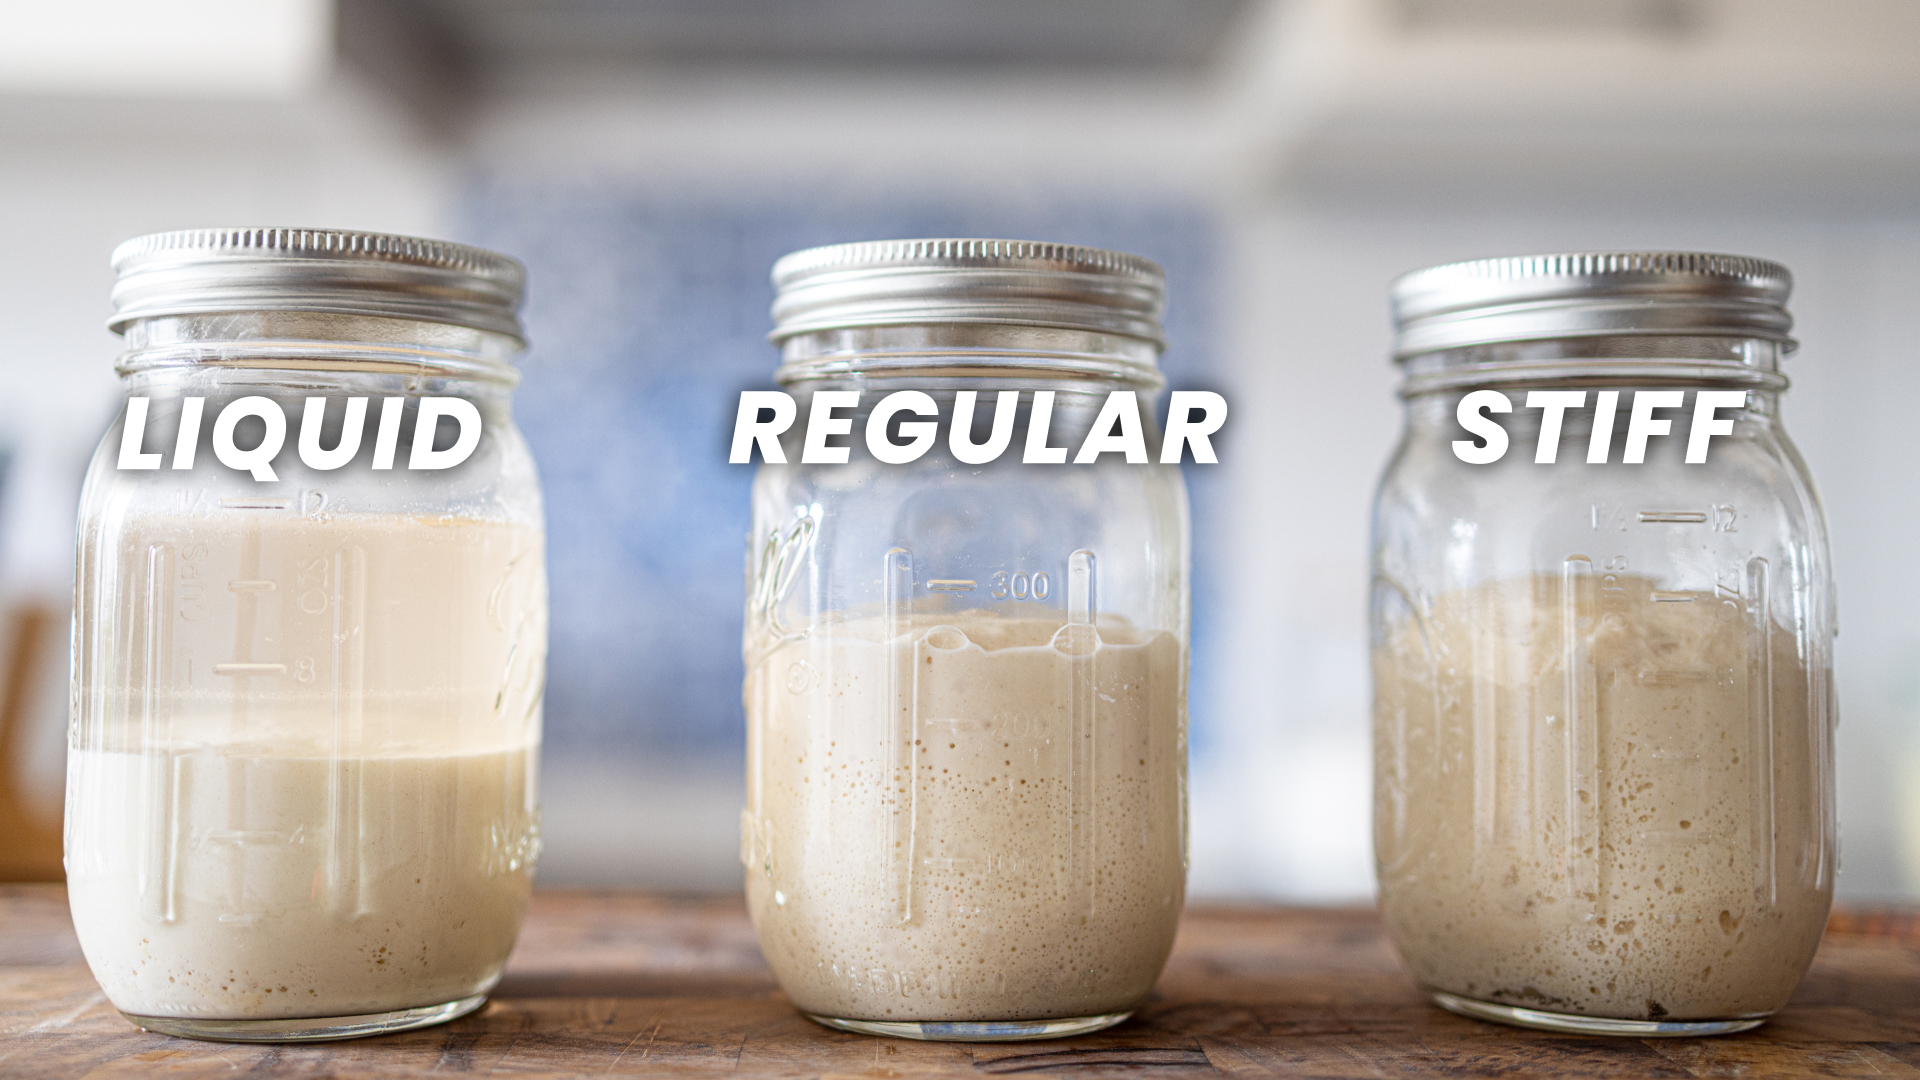
\includegraphics[width=\textwidth]{sourdough-starter-types}
  \caption{3 different starter types next to each other. Note how the liquid starter is submerged
  in water. It has a hydration of 500 percent or more.
  The regular starter has a hydration of around 100 percent, the stiff starter
around 50 to 60 percent.}%
  \label{fig:starter-types}
\end{figure}


You can change your starter type by just adjusting the feeding ratio of how
much flour and water you use. I~frequently change my starter type from
regular to liquid and then back to a stiff starter. After changing the
environment of your microbes, apply feedings at the same ratio over a couple of
days so that they can adapt to the new environment. I~typically see
changes after a single feeding, but I~recommend 2 to 3 feedings, one feeding per
day, to see a stronger effect.

Your dough is generally just a big sourdough starter. So your starter is going
to adapt and regrow inside of your main dough. But you can influence the
properties that your starter carries over to your main dough. If you have more
bacterial fermentation, then your dough will also have slightly more bacterial
fermentation. If you have more yeast fermentation, then your main dough will
have slightly more yeast fermentation. This is important to know when you are
working with a more mature unfed starter. Let's say your starter had last been
fed 48 hours ago. Chances are that your bacteria is very active while the
yeast could be dormant. In such a case you can skip feeding your starter
before making another dough. Just use a very tiny amount of starter. For 1000 g
of flour I~would take around 10 g of starter (1 percent in terms of baker's
math). If my starter is very young and had just been fed 6 to 8 hours ago I~might
end up going up to 20 percent of starter. Remember that your dough is nothing
else other than a big starter. It will tremendously help you to figure out
your best next steps.

When using such a low inoculation rate (1 percent), you need to use stronger
flour when making wheat-based doughs. Your flour naturally breaks down due
to enzymatic activity. It might take 24 hours for the starter to re-grow
inside of your bread dough. At the same time, the enzymatic activity might
have caused your gluten to degrade significantly. While this is okay
when looking at your starter, your wheat-based dough will flatten
out during baking and no longer have the typical characteristics (fluffy crumb
structure). A stronger flour with more gluten is thus advised. It allows for
a longer fermentation before most gluten is broken down.

\section{Regular starter}

\begin{figure}[!htb]
  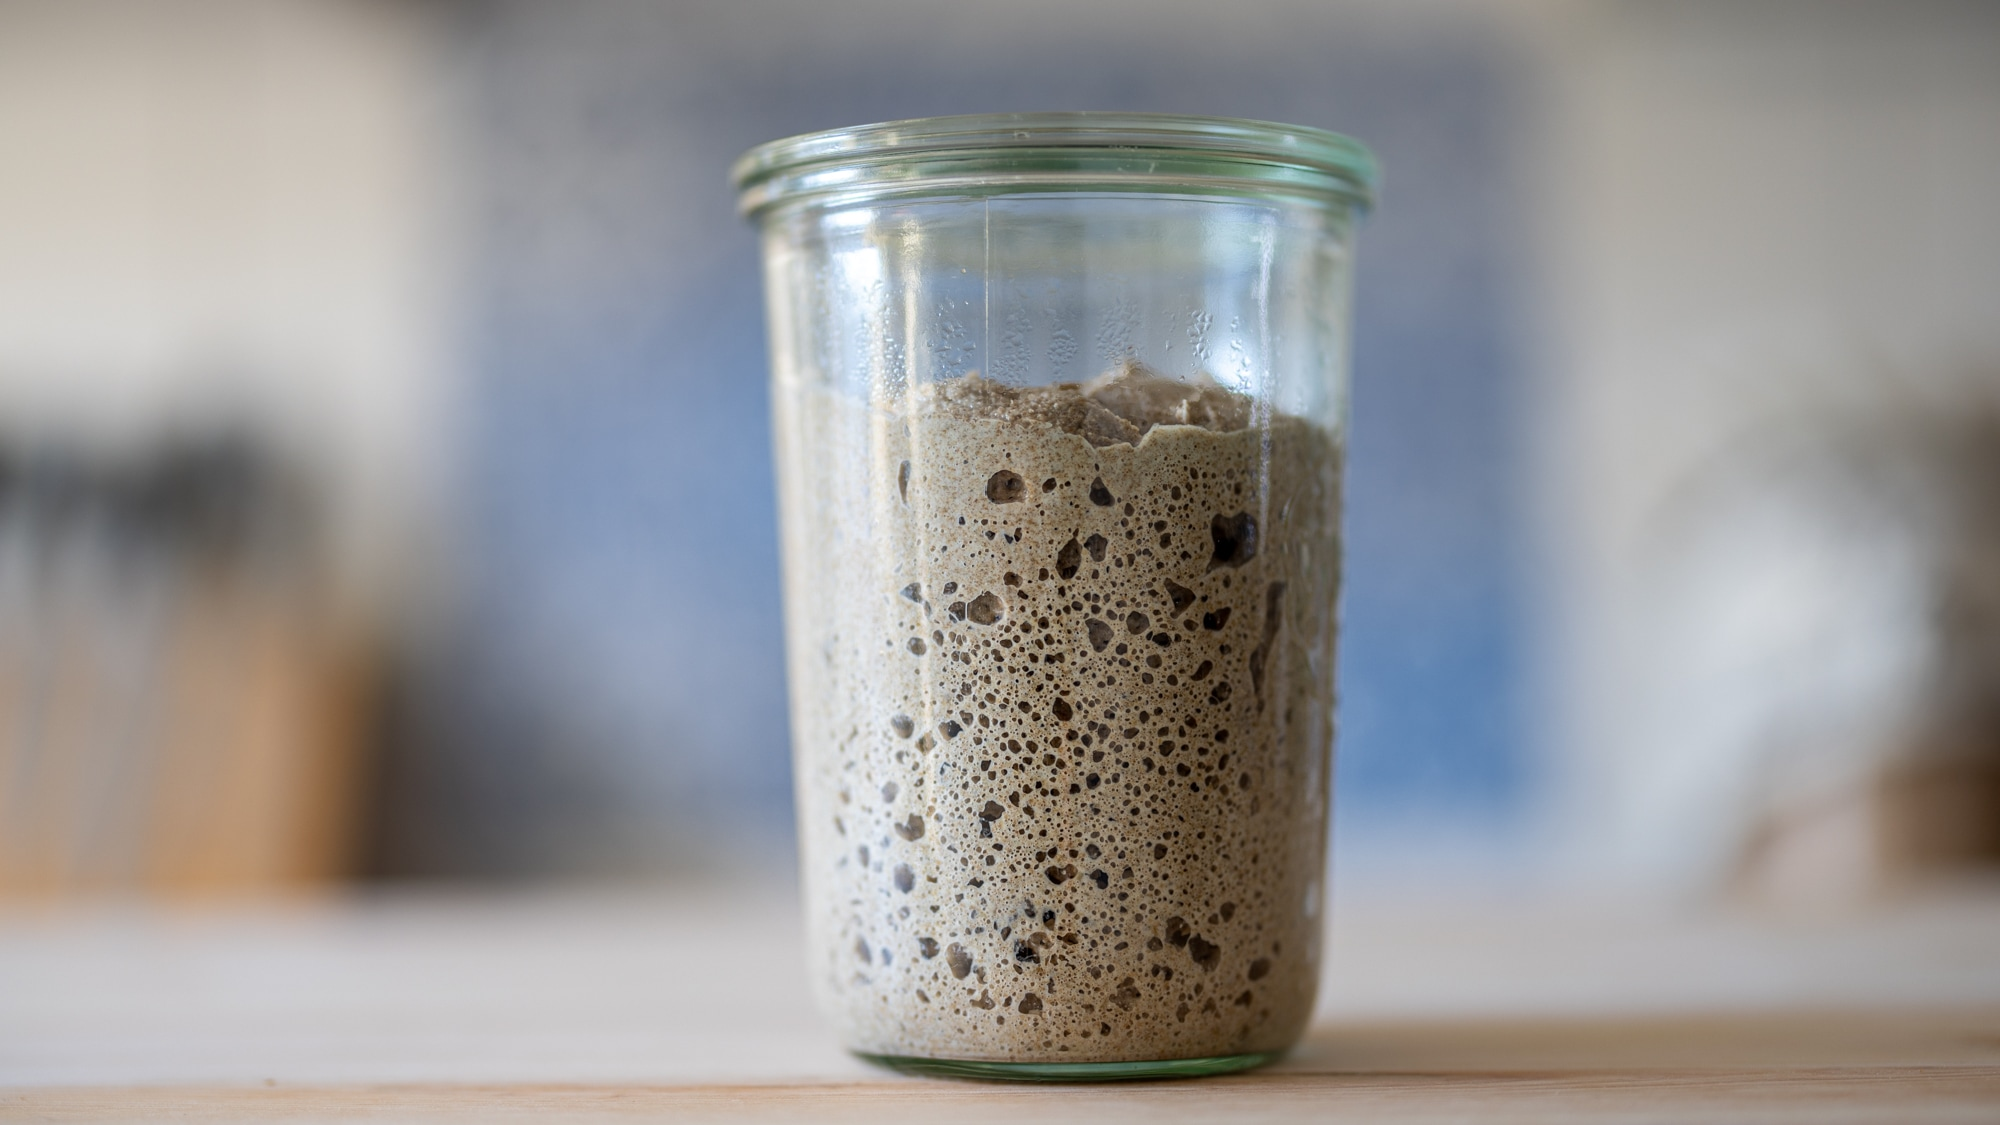
\includegraphics[width=\textwidth]{sourdough-starter.jpg}
  \caption{A regular sourdough starter at 100 percent hydration fed with rye
  flour.}%
  \label{fig:regular-sourdough-starter}
\end{figure}

The regular sourdough starter is made at a hydration of around 100 percent.
This means the starter has equal parts of flour and water. This is the most
common and most universal sourdough starter there is. The starter has a good
balance of yeast and bacteria. After a feeding, the volume increases and
increases. After it reaches a certain peak, it will start to collapse again.

The best way to judge whether the starter is ready is to look at signs such as
air pockets on the edges of your container. Also use the nose to evaluate the
smell of your starter. If you feel that the starter doesn't perform in a
desirable way, chances are that your yeast and bacteria ratios are off. In that
case frequent daily feedings using a 1:5:5 (starter:flour:water) ratio will
help.

A regular starter is a perfect choice to use when utilizing stronger wheat or spelt flours.
It also nicely works with rye, emmer or einkorn. If you only have a weak flour
at hand with less gluten, this starter might cause issues. As you tend to have
quite some bacterial activity, gluten is going to be broken down fast. When
using the starter, use around 1 to 20 percent starter based on the flour of your
dough.

Depending on the bacteria cultivated, a regular starter either has a lactic (dairy),
a vinegary (acetic) or mix of both flavor profiles. You can adjust your
starter's flavor by changing the type to a liquid starter.

\section{Liquid starter}%
\label{section:liquid-starter}

\begin{figure}[!htb]
\begin{center}
  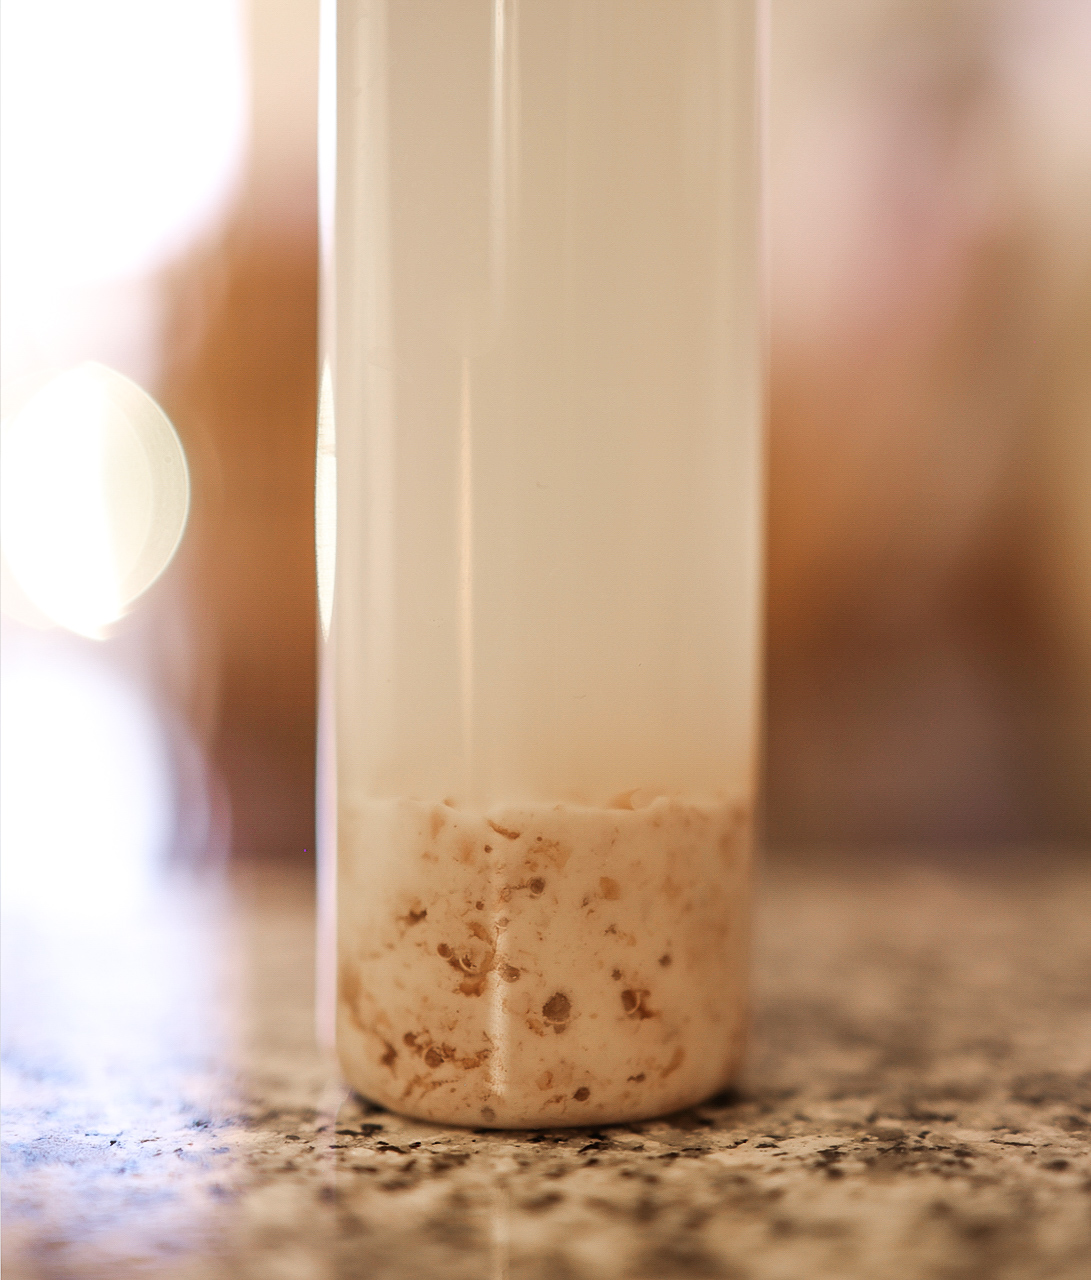
\includegraphics[width=0.5\textwidth]{sourdough-starter-liquid.jpg}
  \caption{A liquid sourdough starter features a high level of water. The high
  water amount boosts lactic acid producing bacteria. After a while the liquid
  and flour start to separate. Bubbles on the side of the flour
  indicate that the starter is ready to be used.}%
  \label{fig:liquid-sourdough-starter}
\end{center}
\end{figure}


\begin{figure}[!htb]
    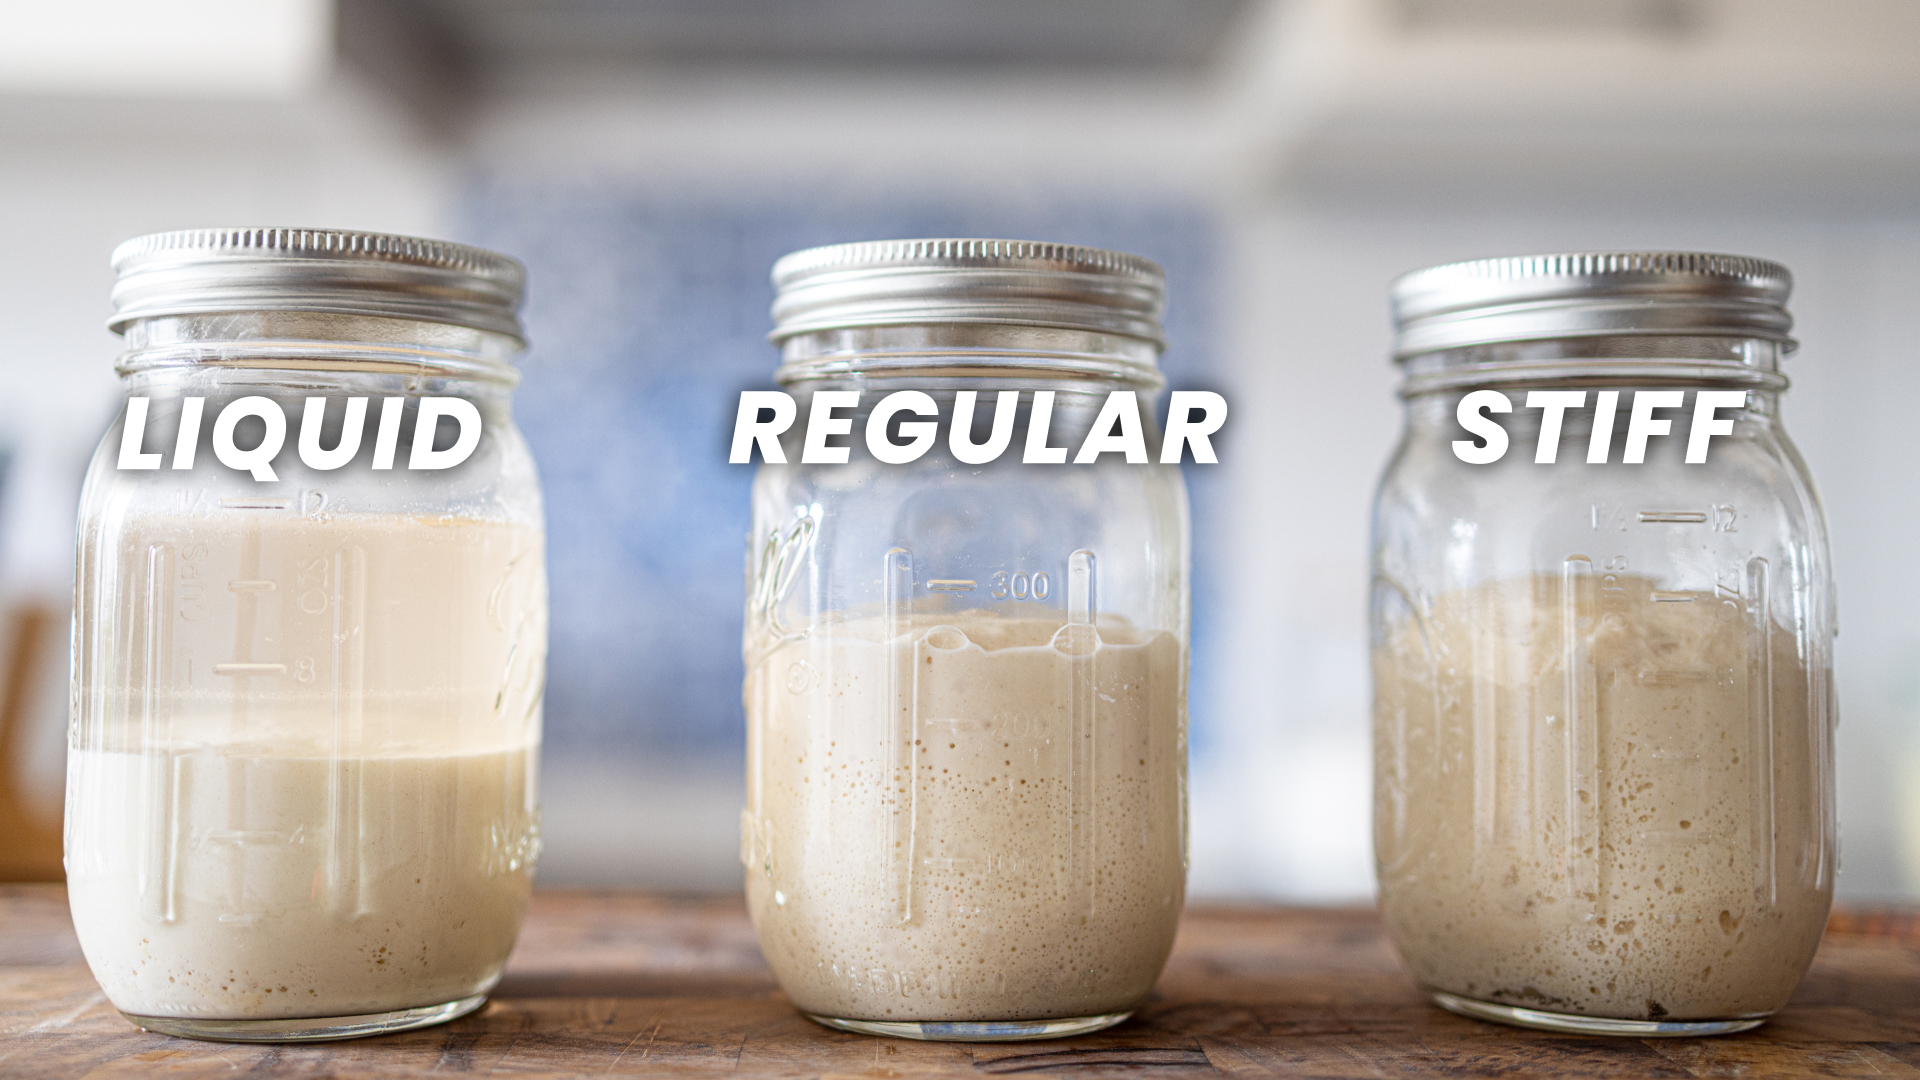
\includegraphics[width=\textwidth]{sourdough-starter-types}
  \caption{3 different starter types next to each other. Note how the liquid starter is submerged
  in water. It has a hydration of 500 percent or more.
  The regular starter has a hydration of around 100 percent, the stiff starter
around 50 to 60 percent.}%
  \label{fig:starter-types}
\end{figure}


You can change your starter type by just adjusting the feeding ratio of how
much flour and water you use. I~frequently change my starter type from
regular to liquid and then back to a stiff starter. After changing the
environment of your microbes, apply feedings at the same ratio over a couple of
days so that they can adapt to the new environment. I~typically see
changes after a single feeding, but I~recommend 2 to 3 feedings, one feeding per
day, to see a stronger effect.

Your dough is generally just a big sourdough starter. So your starter is going
to adapt and regrow inside of your main dough. But you can influence the
properties that your starter carries over to your main dough. If you have more
bacterial fermentation, then your dough will also have slightly more bacterial
fermentation. If you have more yeast fermentation, then your main dough will
have slightly more yeast fermentation. This is important to know when you are
working with a more mature unfed starter. Let's say your starter had last been
fed 48 hours ago. Chances are that your bacteria is very active while the
yeast could be dormant. In such a case you can skip feeding your starter
before making another dough. Just use a very tiny amount of starter. For 1000 g
of flour I~would take around 10 g of starter (1 percent in terms of baker's
math). If my starter is very young and had just been fed 6 to 8 hours ago I~might
end up going up to 20 percent of starter. Remember that your dough is nothing
else other than a big starter. It will tremendously help you to figure out
your best next steps.

When using such a low inoculation rate (1 percent), you need to use stronger
flour when making wheat-based doughs. Your flour naturally breaks down due
to enzymatic activity. It might take 24 hours for the starter to re-grow
inside of your bread dough. At the same time, the enzymatic activity might
have caused your gluten to degrade significantly. While this is okay
when looking at your starter, your wheat-based dough will flatten
out during baking and no longer have the typical characteristics (fluffy crumb
structure). A stronger flour with more gluten is thus advised. It allows for
a longer fermentation before most gluten is broken down.

\section{Regular starter}

\begin{figure}[!htb]
  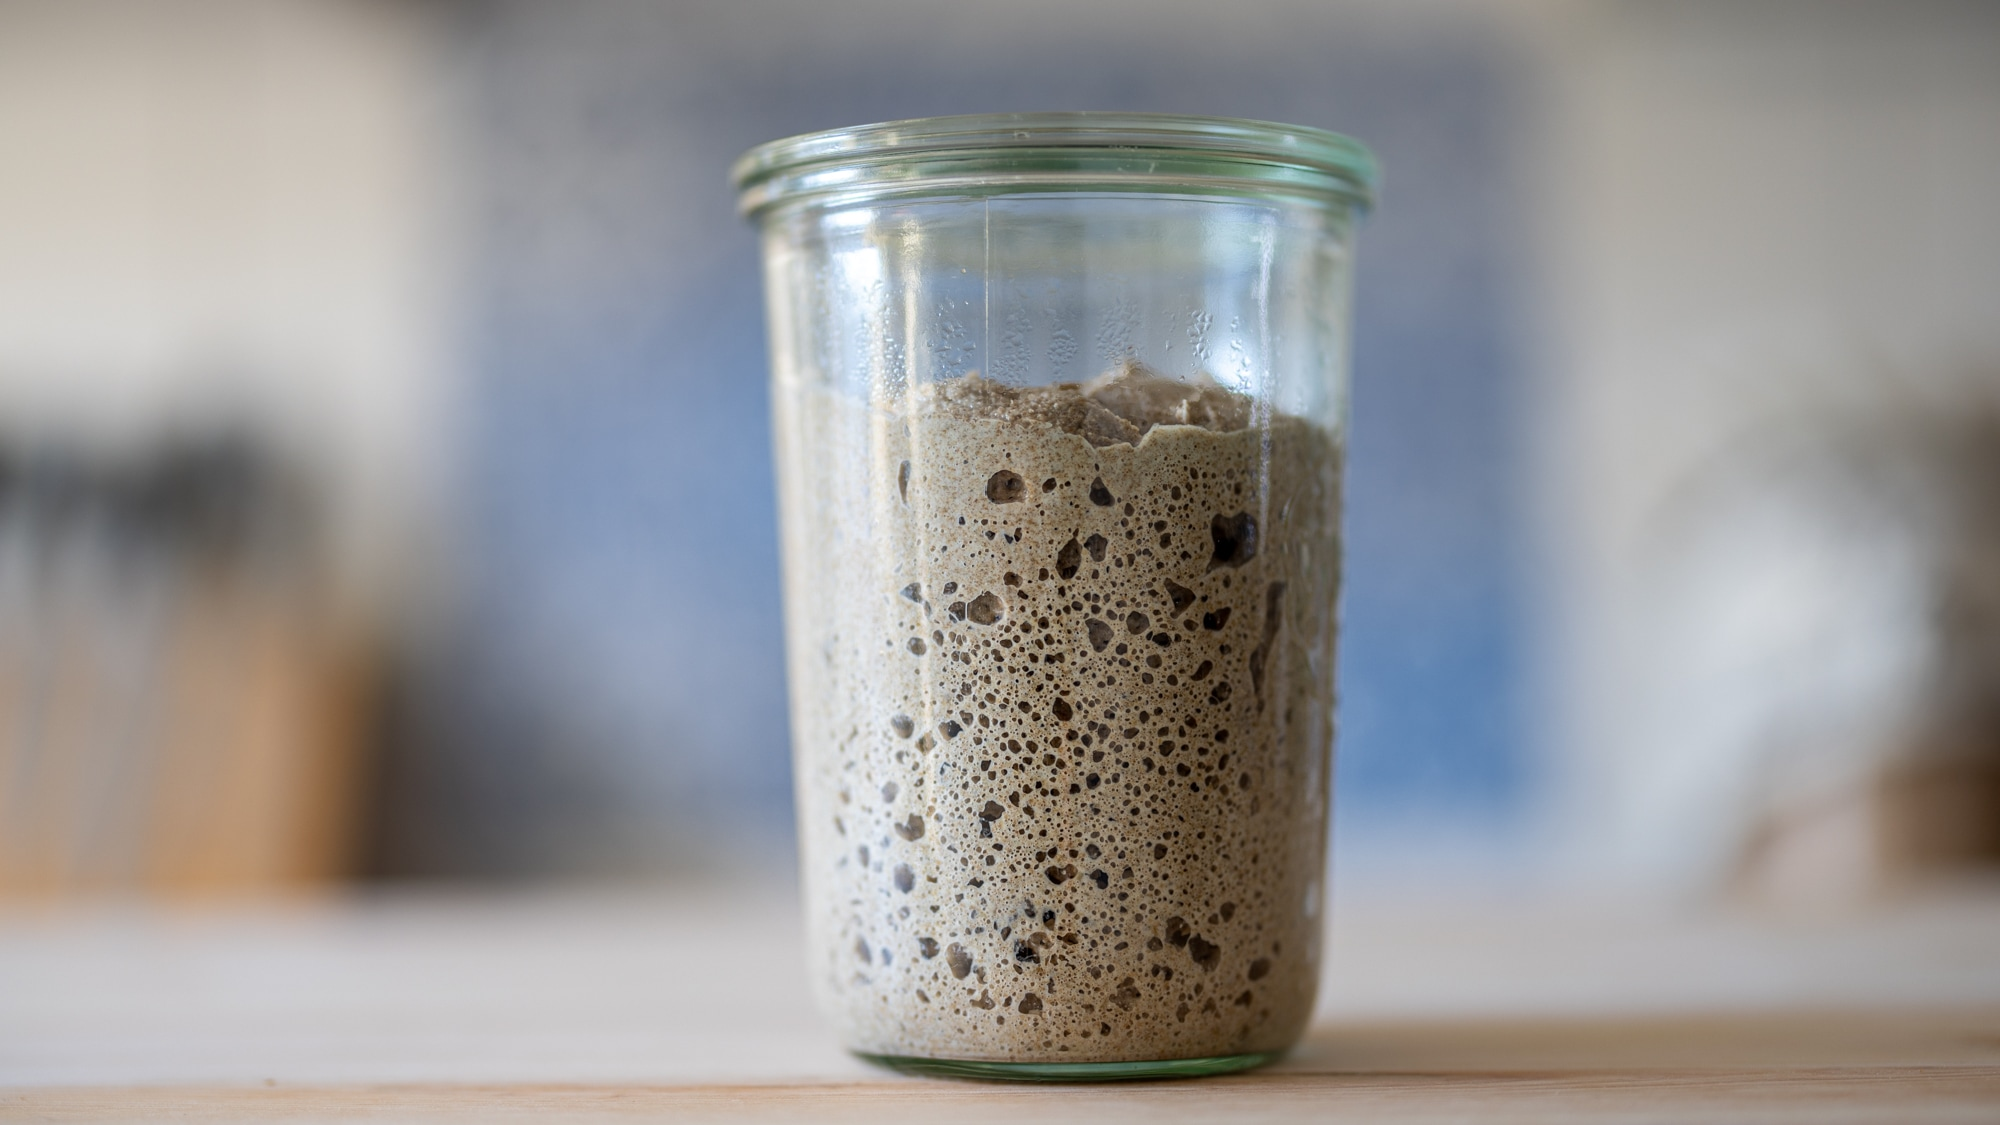
\includegraphics[width=\textwidth]{sourdough-starter.jpg}
  \caption{A regular sourdough starter at 100 percent hydration fed with rye
  flour.}%
  \label{fig:regular-sourdough-starter}
\end{figure}

The regular sourdough starter is made at a hydration of around 100 percent.
This means the starter has equal parts of flour and water. This is the most
common and most universal sourdough starter there is. The starter has a good
balance of yeast and bacteria. After a feeding, the volume increases and
increases. After it reaches a certain peak, it will start to collapse again.

The best way to judge whether the starter is ready is to look at signs such as
air pockets on the edges of your container. Also use the nose to evaluate the
smell of your starter. If you feel that the starter doesn't perform in a
desirable way, chances are that your yeast and bacteria ratios are off. In that
case frequent daily feedings using a 1:5:5 (starter:flour:water) ratio will
help.

A regular starter is a perfect choice to use when utilizing stronger wheat or spelt flours.
It also nicely works with rye, emmer or einkorn. If you only have a weak flour
at hand with less gluten, this starter might cause issues. As you tend to have
quite some bacterial activity, gluten is going to be broken down fast. When
using the starter, use around 1 to 20 percent starter based on the flour of your
dough.

Depending on the bacteria cultivated, a regular starter either has a lactic (dairy),
a vinegary (acetic) or mix of both flavor profiles. You can adjust your
starter's flavor by changing the type to a liquid starter.

\section{Liquid starter}%
\label{section:liquid-starter}

\begin{figure}[!htb]
\begin{center}
  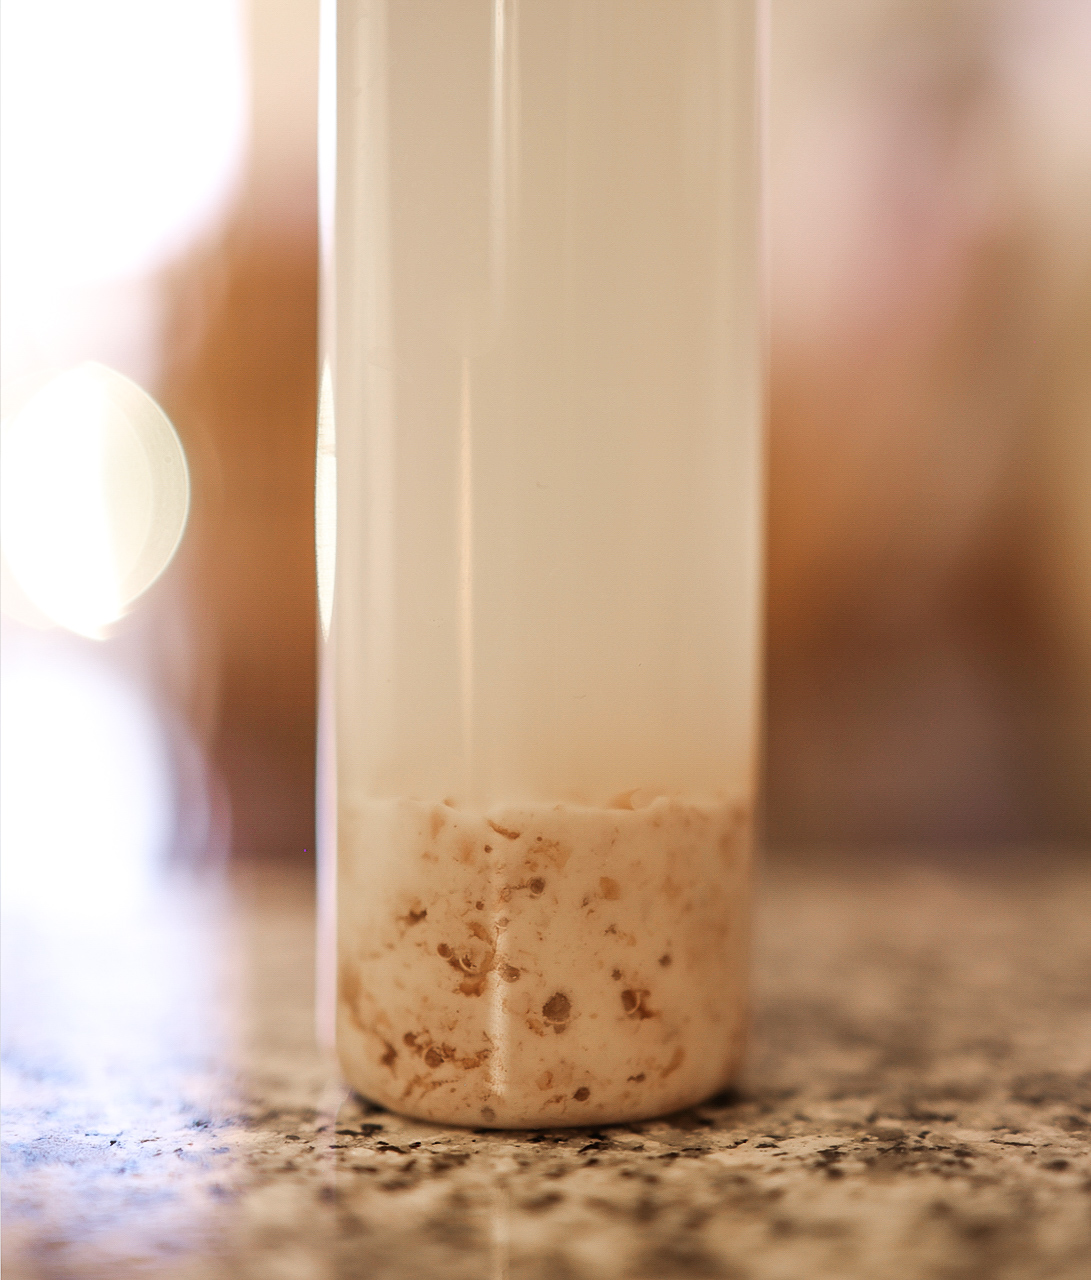
\includegraphics[width=0.5\textwidth]{sourdough-starter-liquid.jpg}
  \caption{A liquid sourdough starter features a high level of water. The high
  water amount boosts lactic acid producing bacteria. After a while the liquid
  and flour start to separate. Bubbles on the side of the flour
  indicate that the starter is ready to be used.}%
  \label{fig:liquid-sourdough-starter}
\end{center}
\end{figure}


\begin{figure}[!htb]
    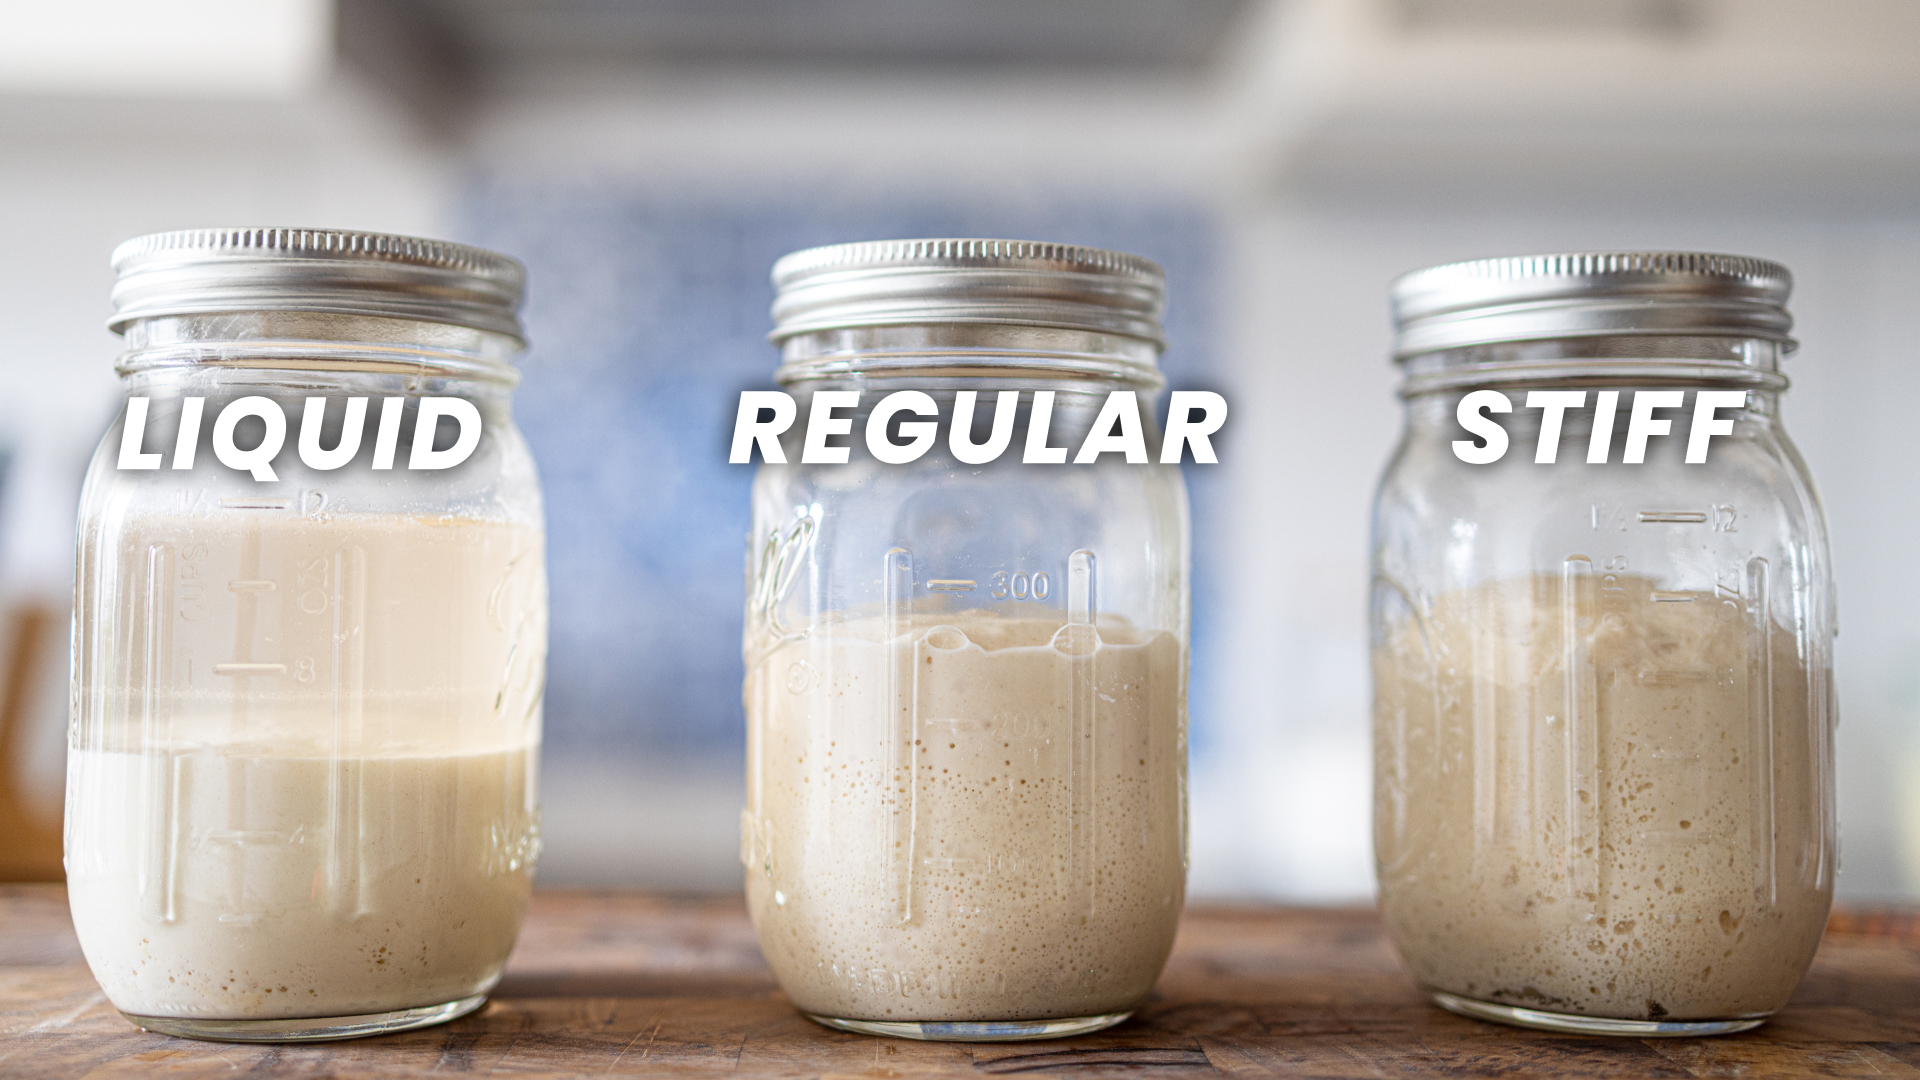
\includegraphics[width=\textwidth]{sourdough-starter-types}
  \caption{3 different starter types next to each other. Note how the liquid starter is submerged
  in water. It has a hydration of 500 percent or more.
  The regular starter has a hydration of around 100 percent, the stiff starter
around 50 to 60 percent.}%
  \label{fig:starter-types}
\end{figure}


You can change your starter type by just adjusting the feeding ratio of how
much flour and water you use. I~frequently change my starter type from
regular to liquid and then back to a stiff starter. After changing the
environment of your microbes, apply feedings at the same ratio over a couple of
days so that they can adapt to the new environment. I~typically see
changes after a single feeding, but I~recommend 2 to 3 feedings, one feeding per
day, to see a stronger effect.

Your dough is generally just a big sourdough starter. So your starter is going
to adapt and regrow inside of your main dough. But you can influence the
properties that your starter carries over to your main dough. If you have more
bacterial fermentation, then your dough will also have slightly more bacterial
fermentation. If you have more yeast fermentation, then your main dough will
have slightly more yeast fermentation. This is important to know when you are
working with a more mature unfed starter. Let's say your starter had last been
fed 48 hours ago. Chances are that your bacteria is very active while the
yeast could be dormant. In such a case you can skip feeding your starter
before making another dough. Just use a very tiny amount of starter. For 1000 g
of flour I~would take around 10 g of starter (1 percent in terms of baker's
math). If my starter is very young and had just been fed 6 to 8 hours ago I~might
end up going up to 20 percent of starter. Remember that your dough is nothing
else other than a big starter. It will tremendously help you to figure out
your best next steps.

When using such a low inoculation rate (1 percent), you need to use stronger
flour when making wheat-based doughs. Your flour naturally breaks down due
to enzymatic activity. It might take 24 hours for the starter to re-grow
inside of your bread dough. At the same time, the enzymatic activity might
have caused your gluten to degrade significantly. While this is okay
when looking at your starter, your wheat-based dough will flatten
out during baking and no longer have the typical characteristics (fluffy crumb
structure). A stronger flour with more gluten is thus advised. It allows for
a longer fermentation before most gluten is broken down.

\section{Regular starter}

\begin{figure}[!htb]
  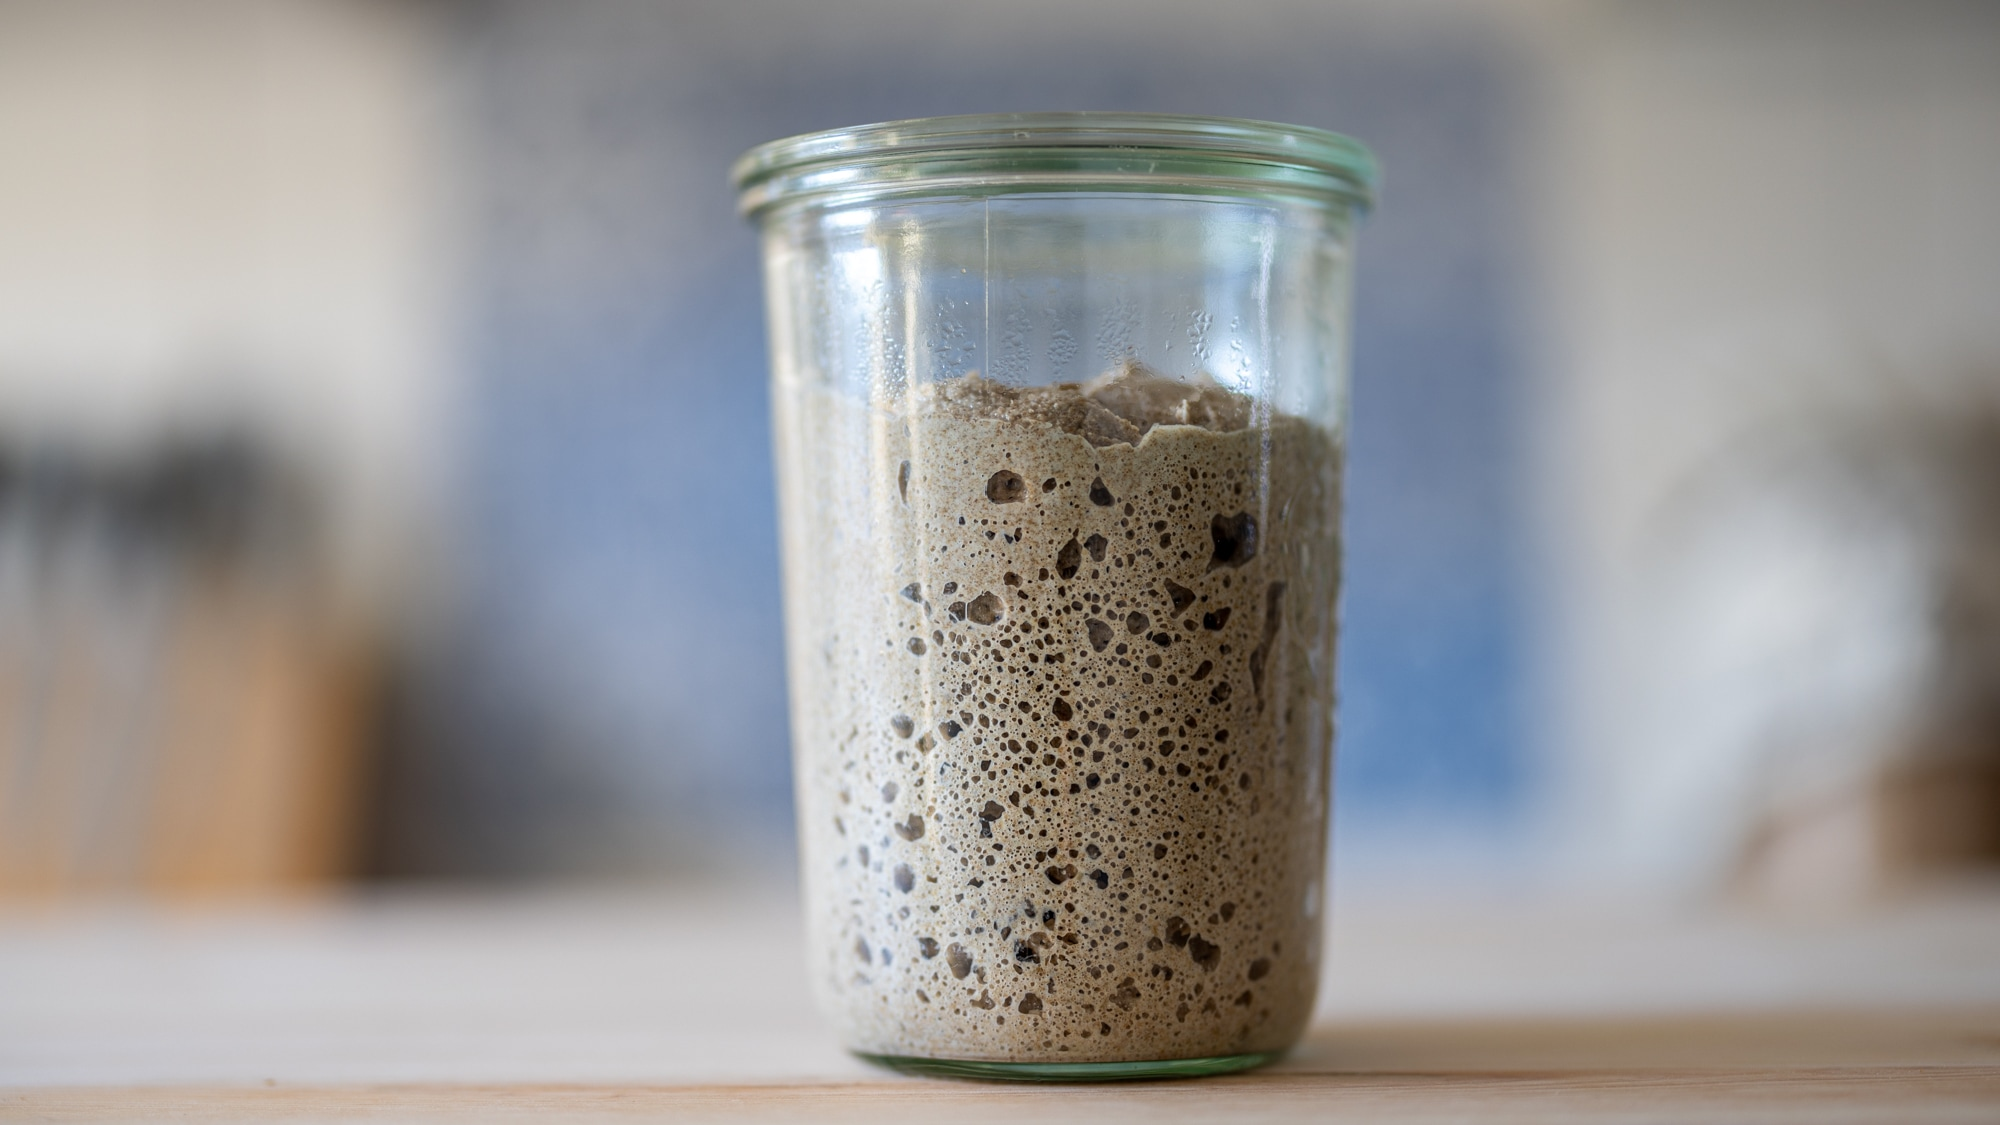
\includegraphics[width=\textwidth]{sourdough-starter.jpg}
  \caption{A regular sourdough starter at 100 percent hydration fed with rye
  flour.}%
  \label{fig:regular-sourdough-starter}
\end{figure}

The regular sourdough starter is made at a hydration of around 100 percent.
This means the starter has equal parts of flour and water. This is the most
common and most universal sourdough starter there is. The starter has a good
balance of yeast and bacteria. After a feeding, the volume increases and
increases. After it reaches a certain peak, it will start to collapse again.

The best way to judge whether the starter is ready is to look at signs such as
air pockets on the edges of your container. Also use the nose to evaluate the
smell of your starter. If you feel that the starter doesn't perform in a
desirable way, chances are that your yeast and bacteria ratios are off. In that
case frequent daily feedings using a 1:5:5 (starter:flour:water) ratio will
help.

A regular starter is a perfect choice to use when utilizing stronger wheat or spelt flours.
It also nicely works with rye, emmer or einkorn. If you only have a weak flour
at hand with less gluten, this starter might cause issues. As you tend to have
quite some bacterial activity, gluten is going to be broken down fast. When
using the starter, use around 1 to 20 percent starter based on the flour of your
dough.

Depending on the bacteria cultivated, a regular starter either has a lactic (dairy),
a vinegary (acetic) or mix of both flavor profiles. You can adjust your
starter's flavor by changing the type to a liquid starter.

\section{Liquid starter}%
\label{section:liquid-starter}

\begin{figure}[!htb]
\begin{center}
  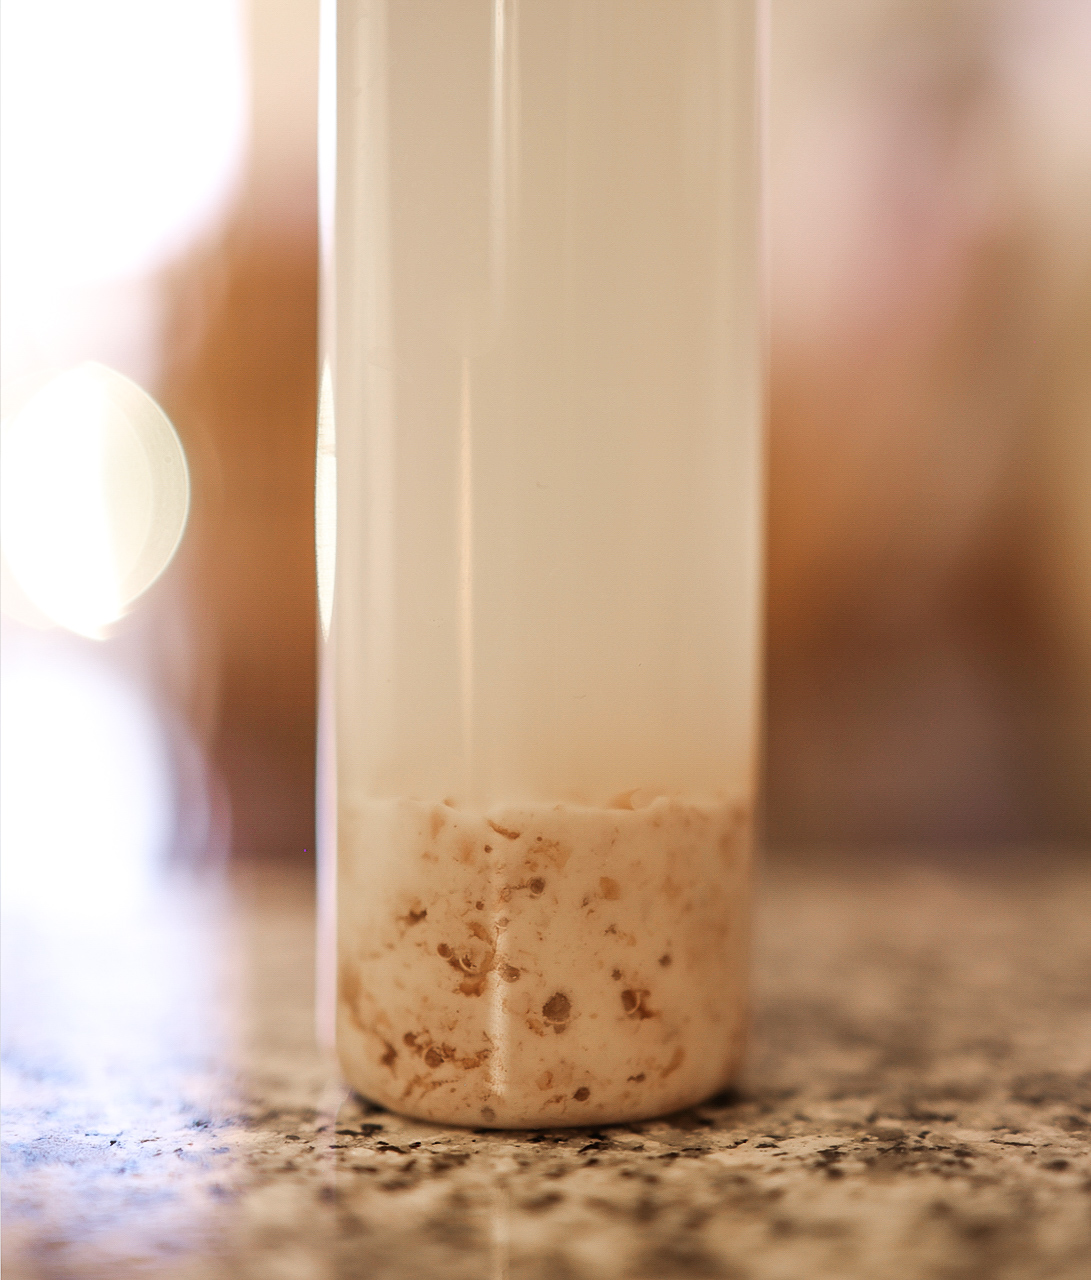
\includegraphics[width=0.5\textwidth]{sourdough-starter-liquid.jpg}
  \caption{A liquid sourdough starter features a high level of water. The high
  water amount boosts lactic acid producing bacteria. After a while the liquid
  and flour start to separate. Bubbles on the side of the flour
  indicate that the starter is ready to be used.}%
  \label{fig:liquid-sourdough-starter}
\end{center}
\end{figure}


\begin{figure}[!htb]
    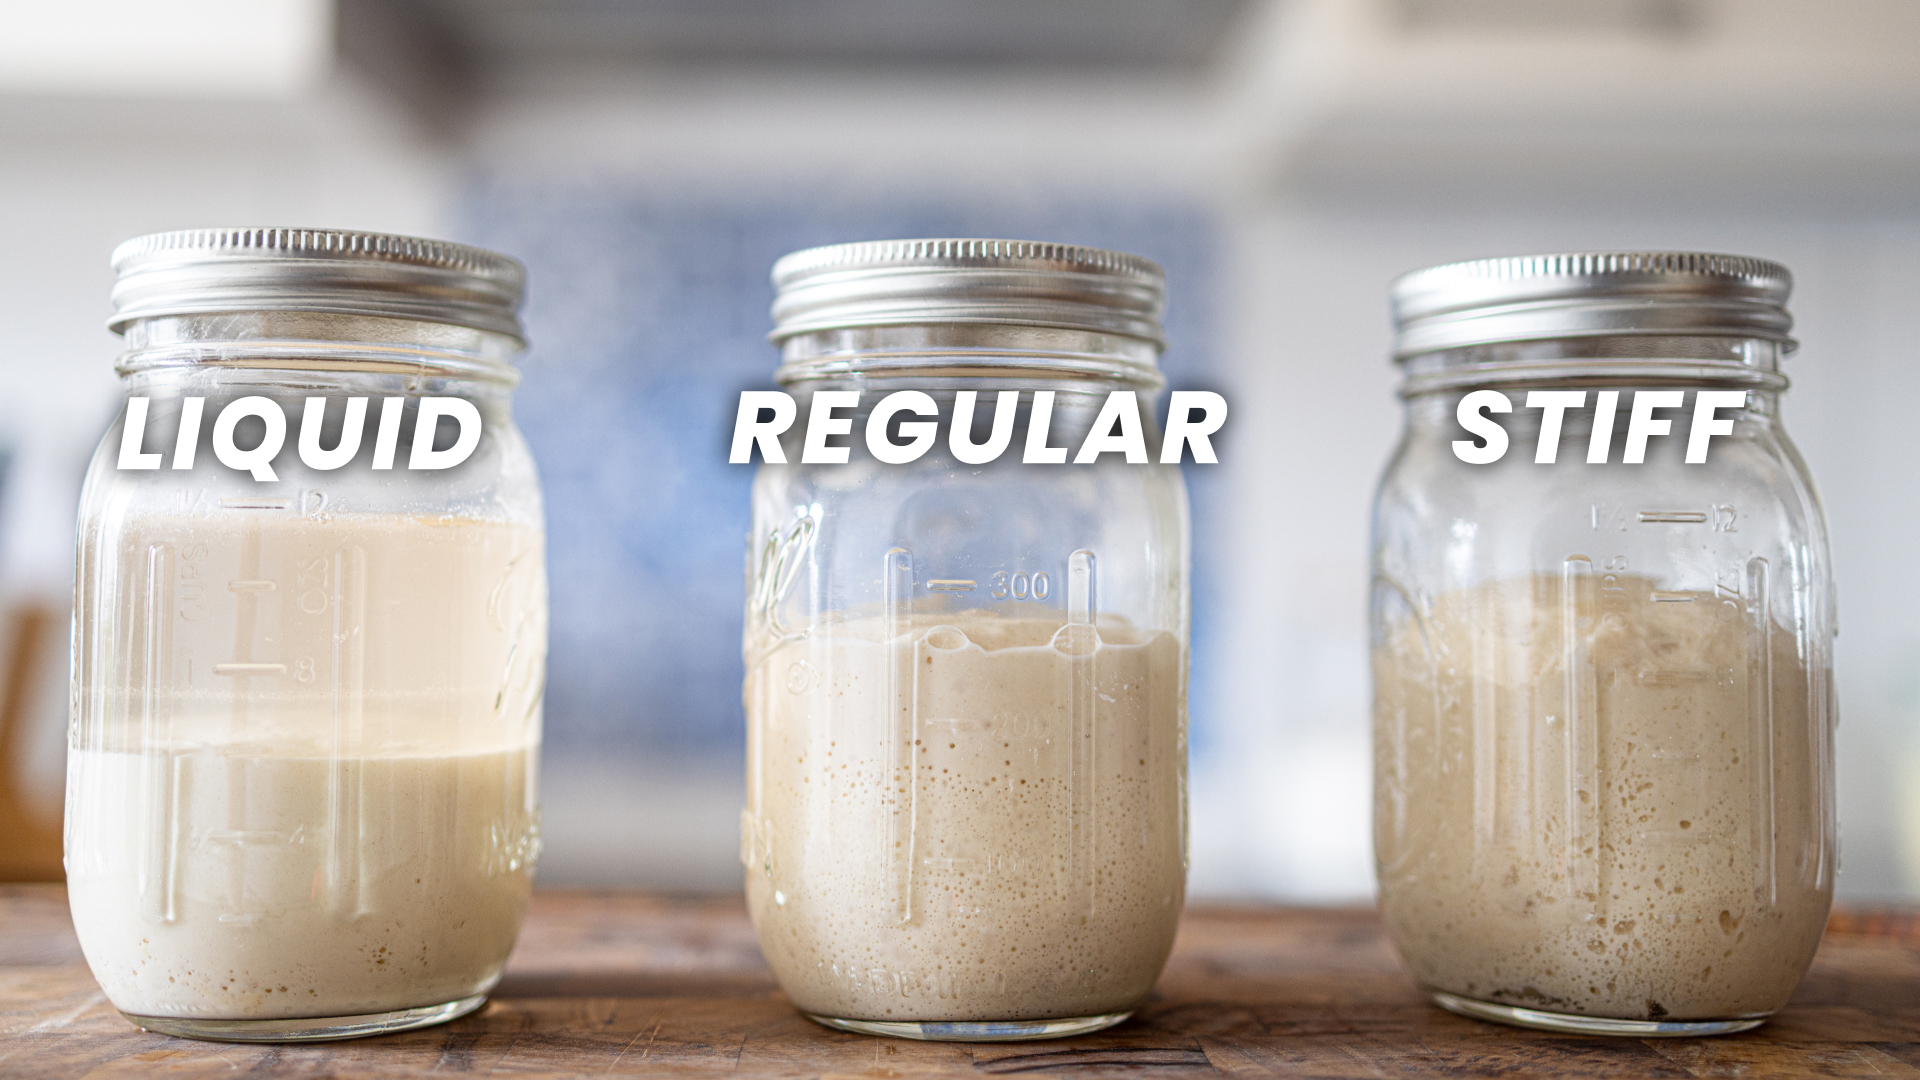
\includegraphics[width=\textwidth]{sourdough-starter-types}
  \caption{3 different starter types next to each other. Note how the liquid starter is submerged
  in water. It has a hydration of 500 percent or more.
  The regular starter has a hydration of around 100 percent, the stiff starter
around 50 to 60 percent.}%
  \label{fig:starter-types}
\end{figure}


You can change your starter type by just adjusting the feeding ratio of how
much flour and water you use. I~frequently change my starter type from
regular to liquid and then back to a stiff starter. After changing the
environment of your microbes, apply feedings at the same ratio over a couple of
days so that they can adapt to the new environment. I~typically see
changes after a single feeding, but I~recommend 2 to 3 feedings, one feeding per
day, to see a stronger effect.

Your dough is generally just a big sourdough starter. So your starter is going
to adapt and regrow inside of your main dough. But you can influence the
properties that your starter carries over to your main dough. If you have more
bacterial fermentation, then your dough will also have slightly more bacterial
fermentation. If you have more yeast fermentation, then your main dough will
have slightly more yeast fermentation. This is important to know when you are
working with a more mature unfed starter. Let's say your starter had last been
fed 48 hours ago. Chances are that your bacteria is very active while the
yeast could be dormant. In such a case you can skip feeding your starter
before making another dough. Just use a very tiny amount of starter. For 1000 g
of flour I~would take around 10 g of starter (1 percent in terms of baker's
math). If my starter is very young and had just been fed 6 to 8 hours ago I~might
end up going up to 20 percent of starter. Remember that your dough is nothing
else other than a big starter. It will tremendously help you to figure out
your best next steps.

When using such a low inoculation rate (1 percent), you need to use stronger
flour when making wheat-based doughs. Your flour naturally breaks down due
to enzymatic activity. It might take 24 hours for the starter to re-grow
inside of your bread dough. At the same time, the enzymatic activity might
have caused your gluten to degrade significantly. While this is okay
when looking at your starter, your wheat-based dough will flatten
out during baking and no longer have the typical characteristics (fluffy crumb
structure). A stronger flour with more gluten is thus advised. It allows for
a longer fermentation before most gluten is broken down.

\section{Regular starter}

\begin{figure}[!htb]
  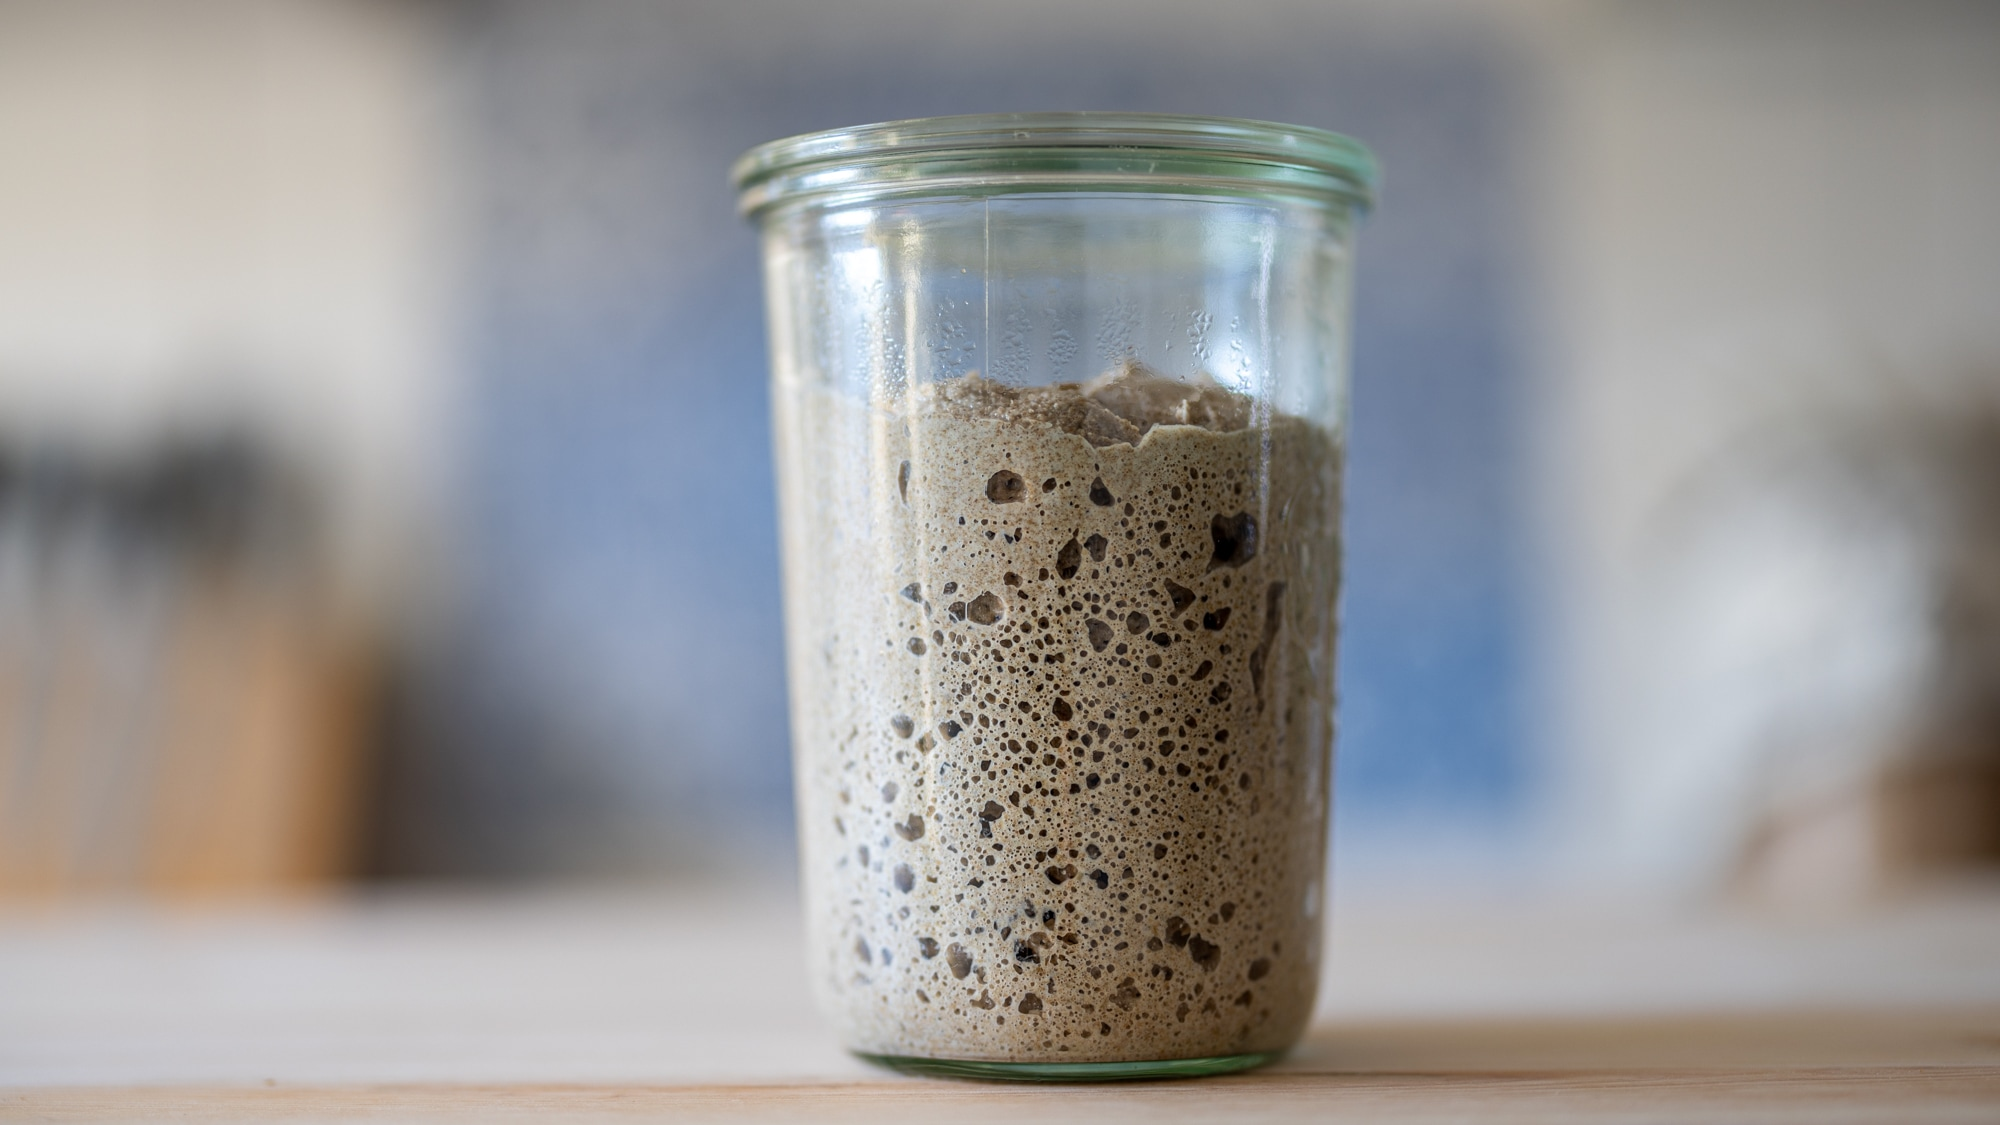
\includegraphics[width=\textwidth]{sourdough-starter.jpg}
  \caption{A regular sourdough starter at 100 percent hydration fed with rye
  flour.}%
  \label{fig:regular-sourdough-starter}
\end{figure}

The regular sourdough starter is made at a hydration of around 100 percent.
This means the starter has equal parts of flour and water. This is the most
common and most universal sourdough starter there is. The starter has a good
balance of yeast and bacteria. After a feeding, the volume increases and
increases. After it reaches a certain peak, it will start to collapse again.

The best way to judge whether the starter is ready is to look at signs such as
air pockets on the edges of your container. Also use the nose to evaluate the
smell of your starter. If you feel that the starter doesn't perform in a
desirable way, chances are that your yeast and bacteria ratios are off. In that
case frequent daily feedings using a 1:5:5 (starter:flour:water) ratio will
help.

A regular starter is a perfect choice to use when utilizing stronger wheat or spelt flours.
It also nicely works with rye, emmer or einkorn. If you only have a weak flour
at hand with less gluten, this starter might cause issues. As you tend to have
quite some bacterial activity, gluten is going to be broken down fast. When
using the starter, use around 1 to 20 percent starter based on the flour of your
dough.

Depending on the bacteria cultivated, a regular starter either has a lactic (dairy),
a vinegary (acetic) or mix of both flavor profiles. You can adjust your
starter's flavor by changing the type to a liquid starter.

\section{Liquid starter}%
\label{section:liquid-starter}

\begin{figure}[!htb]
\begin{center}
  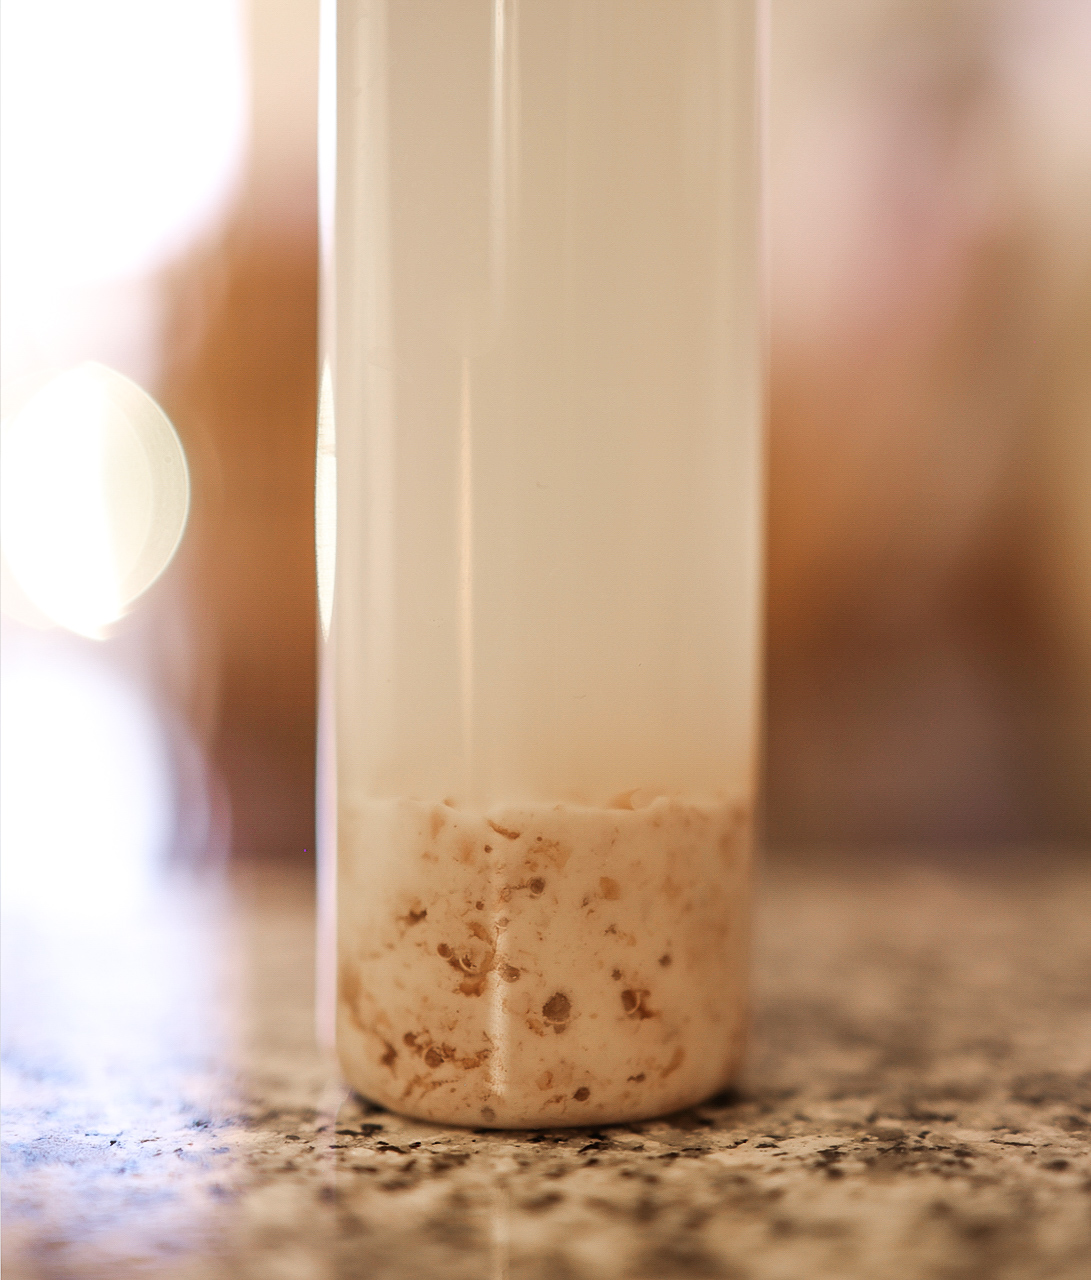
\includegraphics[width=0.5\textwidth]{sourdough-starter-liquid.jpg}
  \caption{A liquid sourdough starter features a high level of water. The high
  water amount boosts lactic acid producing bacteria. After a while the liquid
  and flour start to separate. Bubbles on the side of the flour
  indicate that the starter is ready to be used.}%
  \label{fig:liquid-sourdough-starter}
\end{center}
\end{figure}


\begin{figure}[!htb]
    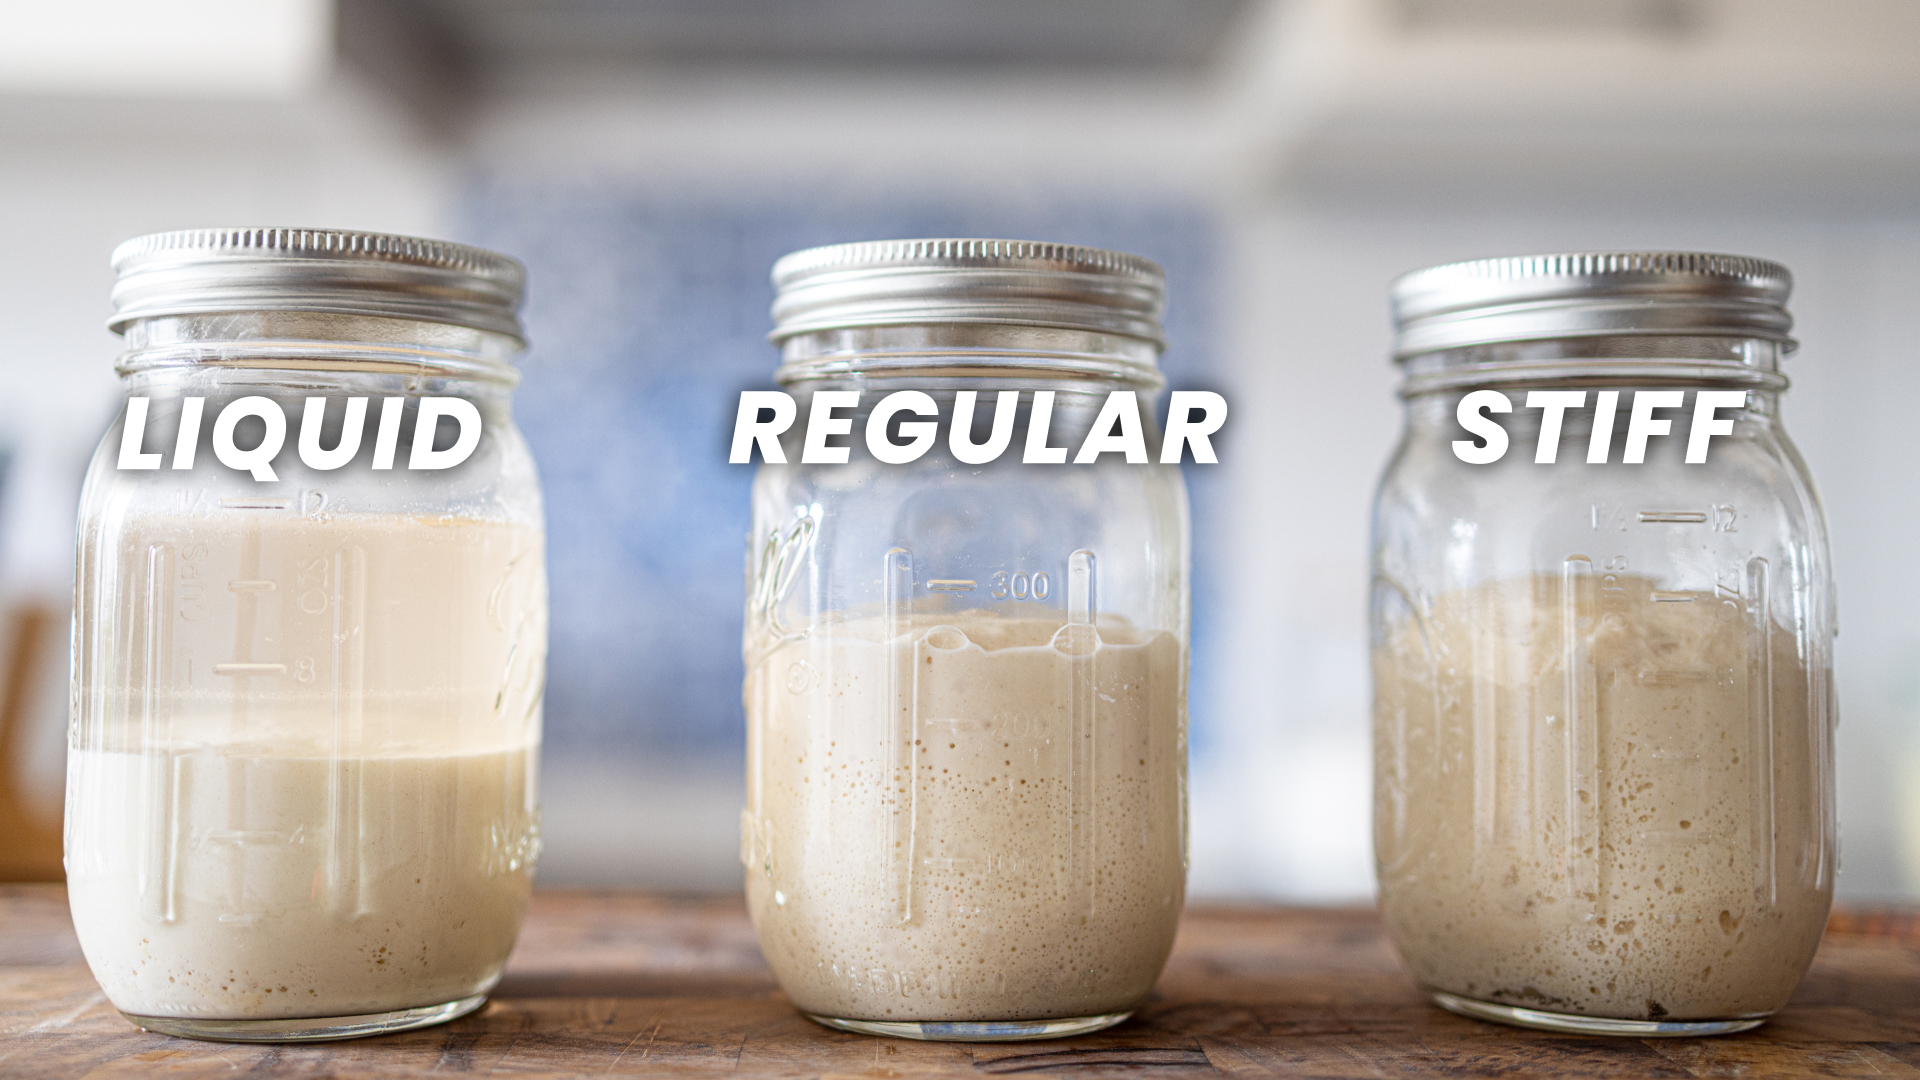
\includegraphics[width=\textwidth]{sourdough-starter-types}
  \caption{3 different starter types next to each other. Note how the liquid starter is submerged
  in water. It has a hydration of 500 percent or more.
  The regular starter has a hydration of around 100 percent, the stiff starter
around 50 to 60 percent.}%
  \label{fig:starter-types}
\end{figure}


You can change your starter type by just adjusting the feeding ratio of how
much flour and water you use. I~frequently change my starter type from
regular to liquid and then back to a stiff starter. After changing the
environment of your microbes, apply feedings at the same ratio over a couple of
days so that they can adapt to the new environment. I~typically see
changes after a single feeding, but I~recommend 2 to 3 feedings, one feeding per
day, to see a stronger effect.

Your dough is generally just a big sourdough starter. So your starter is going
to adapt and regrow inside of your main dough. But you can influence the
properties that your starter carries over to your main dough. If you have more
bacterial fermentation, then your dough will also have slightly more bacterial
fermentation. If you have more yeast fermentation, then your main dough will
have slightly more yeast fermentation. This is important to know when you are
working with a more mature unfed starter. Let's say your starter had last been
fed 48 hours ago. Chances are that your bacteria is very active while the
yeast could be dormant. In such a case you can skip feeding your starter
before making another dough. Just use a very tiny amount of starter. For 1000 g
of flour I~would take around 10 g of starter (1 percent in terms of baker's
math). If my starter is very young and had just been fed 6 to 8 hours ago I~might
end up going up to 20 percent of starter. Remember that your dough is nothing
else other than a big starter. It will tremendously help you to figure out
your best next steps.

When using such a low inoculation rate (1 percent), you need to use stronger
flour when making wheat-based doughs. Your flour naturally breaks down due
to enzymatic activity. It might take 24 hours for the starter to re-grow
inside of your bread dough. At the same time, the enzymatic activity might
have caused your gluten to degrade significantly. While this is okay
when looking at your starter, your wheat-based dough will flatten
out during baking and no longer have the typical characteristics (fluffy crumb
structure). A stronger flour with more gluten is thus advised. It allows for
a longer fermentation before most gluten is broken down.

\section{Regular starter}

\begin{figure}[!htb]
  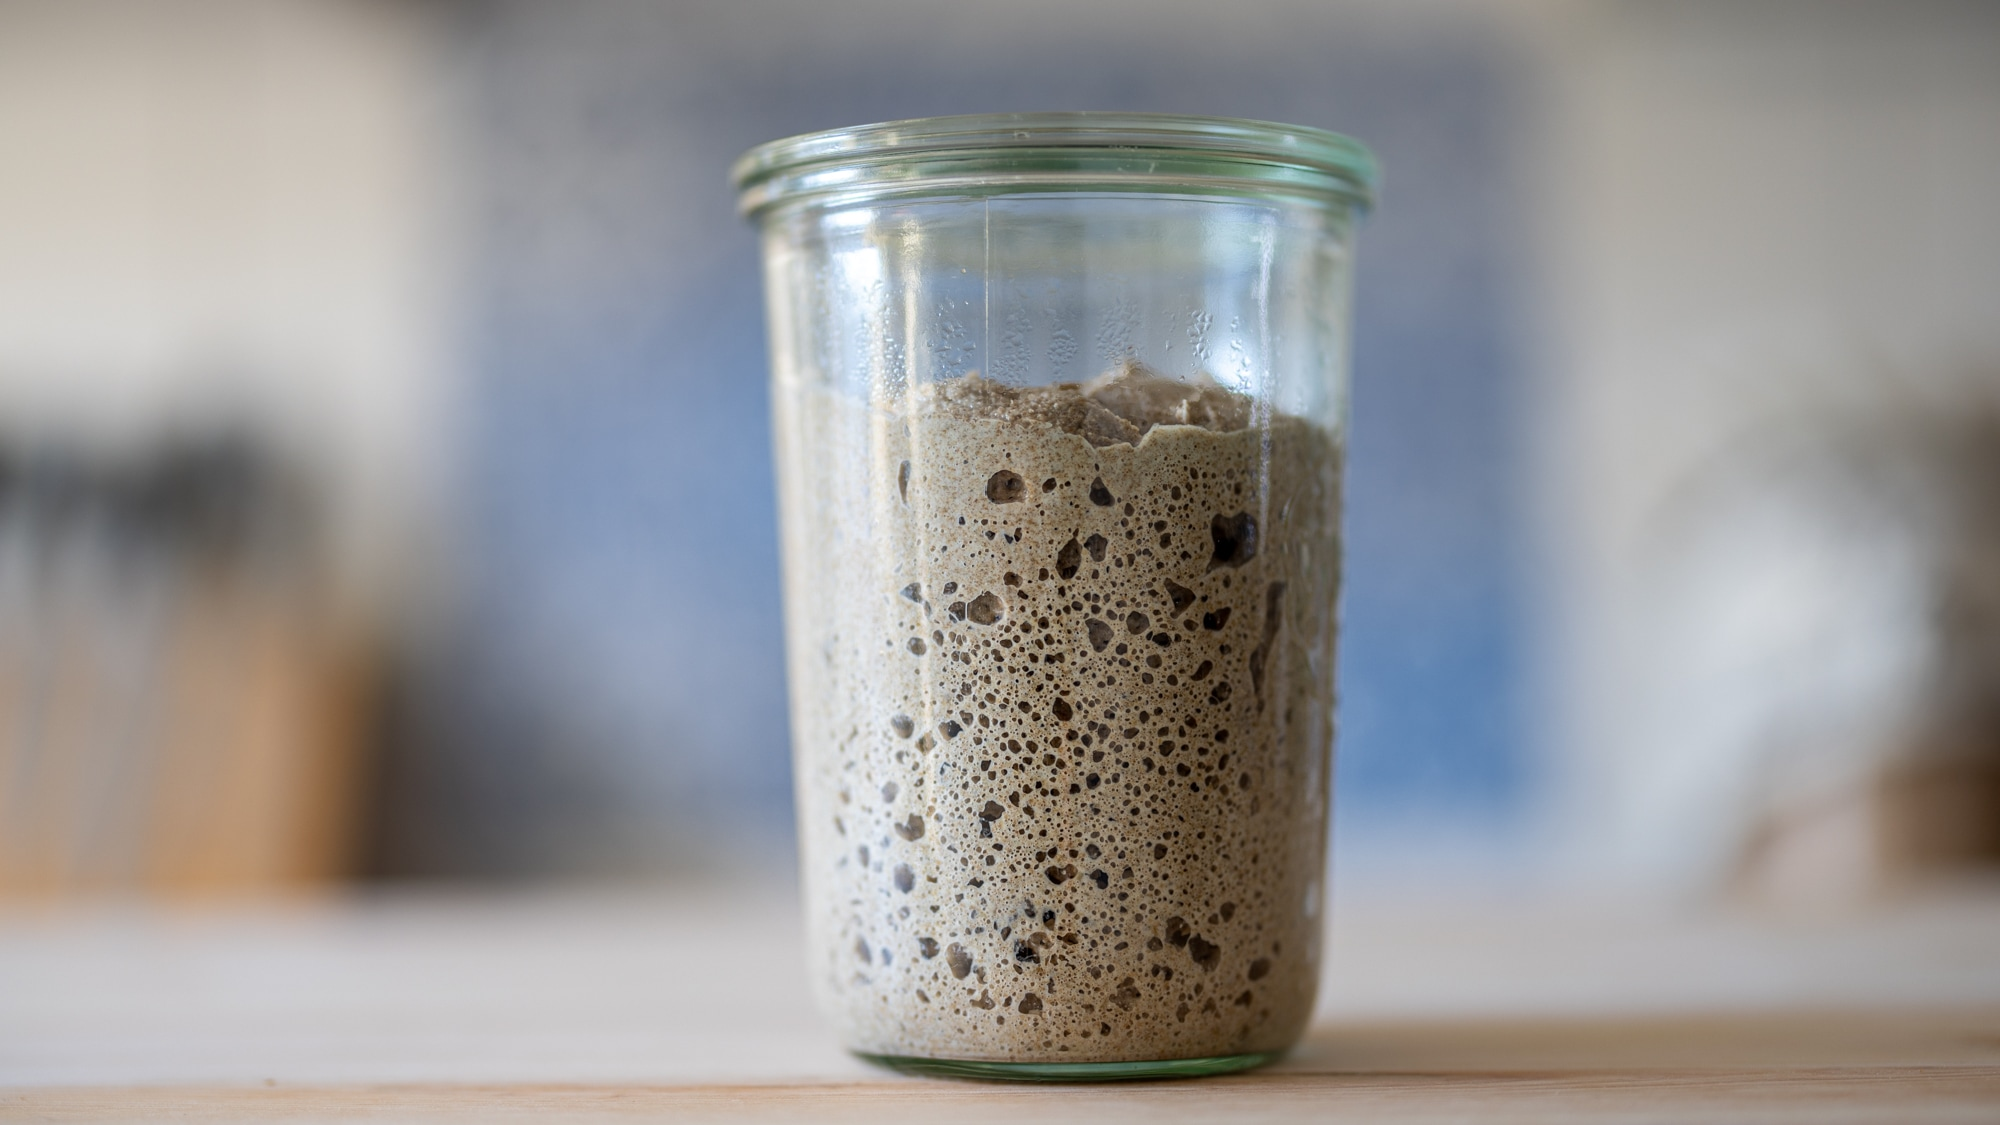
\includegraphics[width=\textwidth]{sourdough-starter.jpg}
  \caption{A regular sourdough starter at 100 percent hydration fed with rye
  flour.}%
  \label{fig:regular-sourdough-starter}
\end{figure}

The regular sourdough starter is made at a hydration of around 100 percent.
This means the starter has equal parts of flour and water. This is the most
common and most universal sourdough starter there is. The starter has a good
balance of yeast and bacteria. After a feeding, the volume increases and
increases. After it reaches a certain peak, it will start to collapse again.

The best way to judge whether the starter is ready is to look at signs such as
air pockets on the edges of your container. Also use the nose to evaluate the
smell of your starter. If you feel that the starter doesn't perform in a
desirable way, chances are that your yeast and bacteria ratios are off. In that
case frequent daily feedings using a 1:5:5 (starter:flour:water) ratio will
help.

A regular starter is a perfect choice to use when utilizing stronger wheat or spelt flours.
It also nicely works with rye, emmer or einkorn. If you only have a weak flour
at hand with less gluten, this starter might cause issues. As you tend to have
quite some bacterial activity, gluten is going to be broken down fast. When
using the starter, use around 1 to 20 percent starter based on the flour of your
dough.

Depending on the bacteria cultivated, a regular starter either has a lactic (dairy),
a vinegary (acetic) or mix of both flavor profiles. You can adjust your
starter's flavor by changing the type to a liquid starter.

\section{Liquid starter}%
\label{section:liquid-starter}

\begin{figure}[!htb]
\begin{center}
  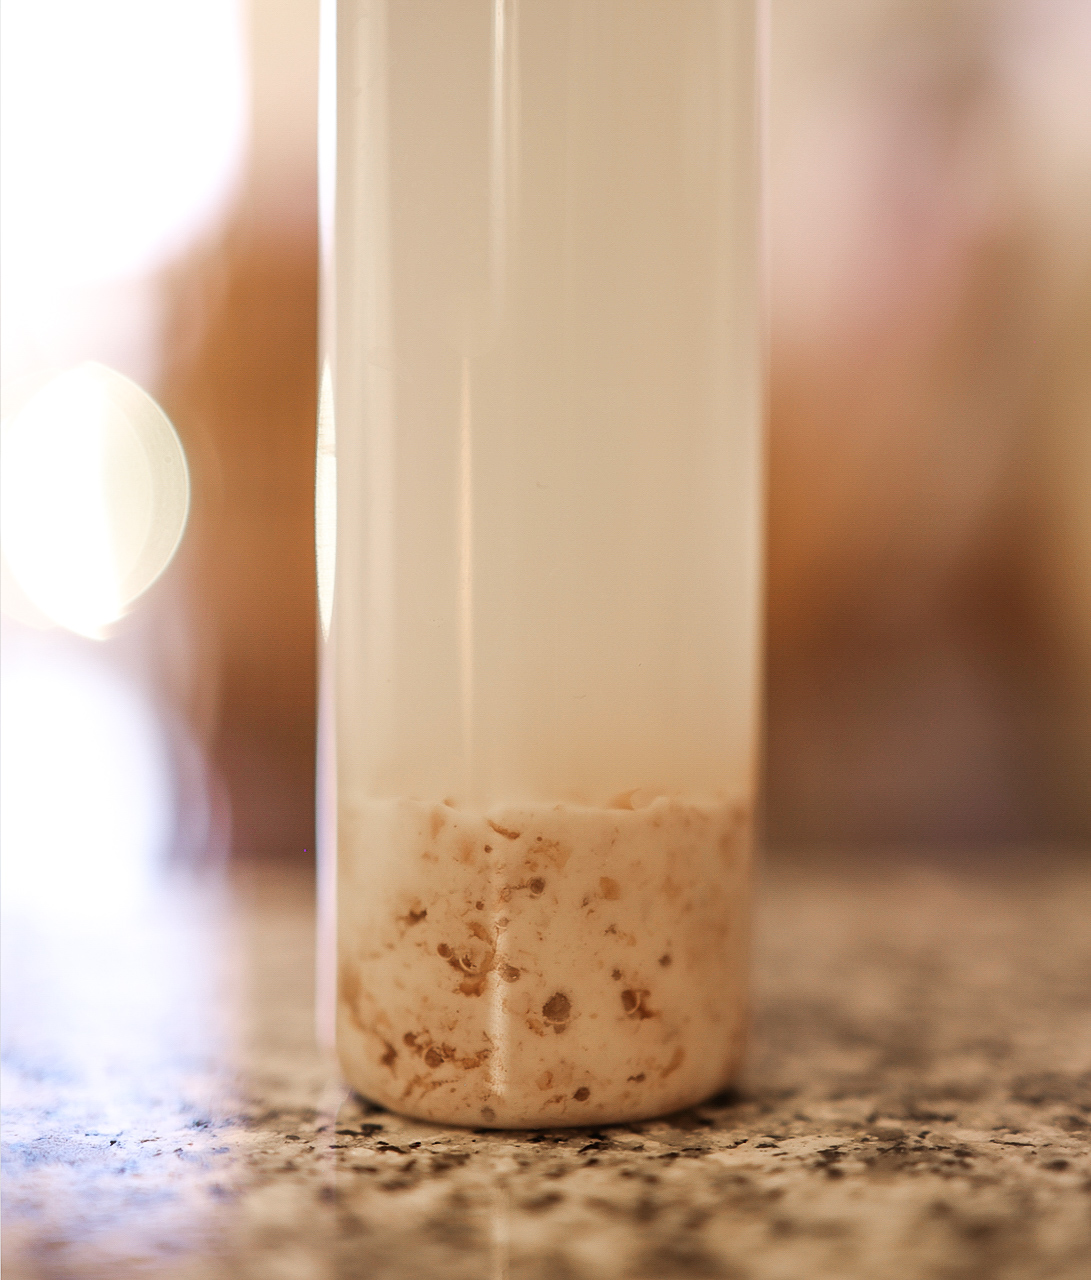
\includegraphics[width=0.5\textwidth]{sourdough-starter-liquid.jpg}
  \caption{A liquid sourdough starter features a high level of water. The high
  water amount boosts lactic acid producing bacteria. After a while the liquid
  and flour start to separate. Bubbles on the side of the flour
  indicate that the starter is ready to be used.}%
  \label{fig:liquid-sourdough-starter}
\end{center}
\end{figure}


\begin{figure}[!htb]
\begin{center}
  \begin{tikzpicture}[node distance = 3cm, auto]
  \node [start] (init) {Make a regular or stiff starter};
  \node [block, right of=init] (feed_new_ratio) {Mix \qty{1}{\gram} existing starter, \qty{5}{\gram} flour and \qty{25}{\gram} water};
  \node [block, right of=feed_new_ratio] (next_day) {Wait\\ \qty{24}{\hour}};
  \node [block, below of=init, node distance=4cm] (feed_again) {Feed again using 1:5:25 ratio};
  \node [block, right of=next_day, node distance=5cm] (test) {Check starter readiness?};
  \node [decision, below of=next_day, node distance=4cm] (ready_signs) {Sour yogurty smell and bubbles visible on flour?};
  \node [block, below of=test, node distance=4cm] (last_feed) {Feed one last time};
  \node [success, below of=last_feed, node distance=3cm] (bread_dough) {Make bread dough};
  \path [line] (init) -- (feed_new_ratio);
  \path [line] (feed_new_ratio) -- (next_day);
  \path [line] (feed_again) -- node{repeat 3 times} (feed_new_ratio);
  \path [line] (next_day) -- node{after 3~days} (test);
  \path [line] (next_day) -- (feed_again);
  \path [line] (test) -- (ready_signs);
  \path [line] (ready_signs) -- node{no} (feed_again);
  \path [line] (ready_signs) -- node{yes} (last_feed);
  \path [line] (last_feed) -- node{after \qtyrange{6}{12}{\hour}} (bread_dough);
\end{tikzpicture}

  \caption{The process to convert your regular or stiff starter into a liquid starter. The whole
  process takes around 3 days. The longer you maintain your starter at the
  suggested hydration level, the more adapted your microorganisms become. It is recommended
  to keep a backup of your original starter as the liquid environment will select
  anaerobic microorganisms. This boosts bacteria that create lactic acid rather
  than acetic acid. The resulting acidity will be perceived as milder.}%
  \label{fig:liquid-starter-conversion}
\end{center}
\end{figure}

The liquid starter is made at a hydration of around 500 percent. This means
the starter has much more water than flour. The additional layer of water on
top of the flour changes the microbiome of your starter.

By introducing this layer of water, less oxygen is available throughout the
course of fermentation. This means that your starter will no longer be
producing acetic acid. The heterofermentative lactic acid bacteria will thrive
in this environment. This is a neat little trick to change your starter's
flavor profile from vinegary to lactic. Your starter is going to develop
dairy creamy notes. Interestingly, when changing the hydration again, your starter
is going to maintain the liquid starter flavor profile, but then benefit again
from enhanced yeast activity. The liquid starter conversion is non reversible.
So ideally keep a backup of your stiff or regular starter.

To commence with the
conversion, simply take around 1 gram of your starter, mix with 5 g flour and
25 g water. Stir everything together properly. After a few minutes the flour is
going to start settling in at the bottom of your jar. Repeat this process over
a few days. Shake the starter gently to see if you can see tiny \ch{CO2} bubbles
moving in the liquid. This is a good sign that your starter is ready. Use your
nose to smell the starter. It should have a creamy dairy flavor note.

As you have more bacterial activity, this starter works best with a very strong
flour that can withstand a long fermentation period. Using this starter with a
weak wheat flour will not work. If you do not care about baking a freestanding loaf,
then you can easily use this starter together with a loaf pan.
This starter also works great when making a hearty pancake dough. To use it
I~shake the starter container until I~see all ingredients are homogenized.  Then
I~use around 5 percent of it in terms of baker's math. So for 1000 g of flour
that's around 50 grams of liquid starter. As it is very liquid you have to
include the 50 grams in your liquid calculation. I~typically treat the starter
directly as liquid in the recipes. So if the recipe calls for 600 grams of water
and I~use 50 grams of starter, then I~would proceed and only use 550 grams of
water.

This type of starter is also an excellent mold combatant. As you are removing
oxygen from the equation, aerobic mold can not properly grow. If your starter
has a mold problem then the liquid conversion could be the remedy. Take a
piece of your starter where you suspect no mold growth. Apply the conversion
as mentioned before. The mold will likely sporulate as it runs out of food.
With each new feeding you are reducing the mold spores. The spores can no
longer reactivate as they can not do so in the anaerobic conditions.

The liquid on top of your starter is an excellent resource that you could use
to make sauces. If you feel you would like to add a little bit of acidity,
drain the liquid part on your starter and use it. I~have used it numerous
times to make lacto-fermented hot sauces.

\section{Stiff starter}%
\label{section:stiff-starter}

\begin{figure}[!htb]
  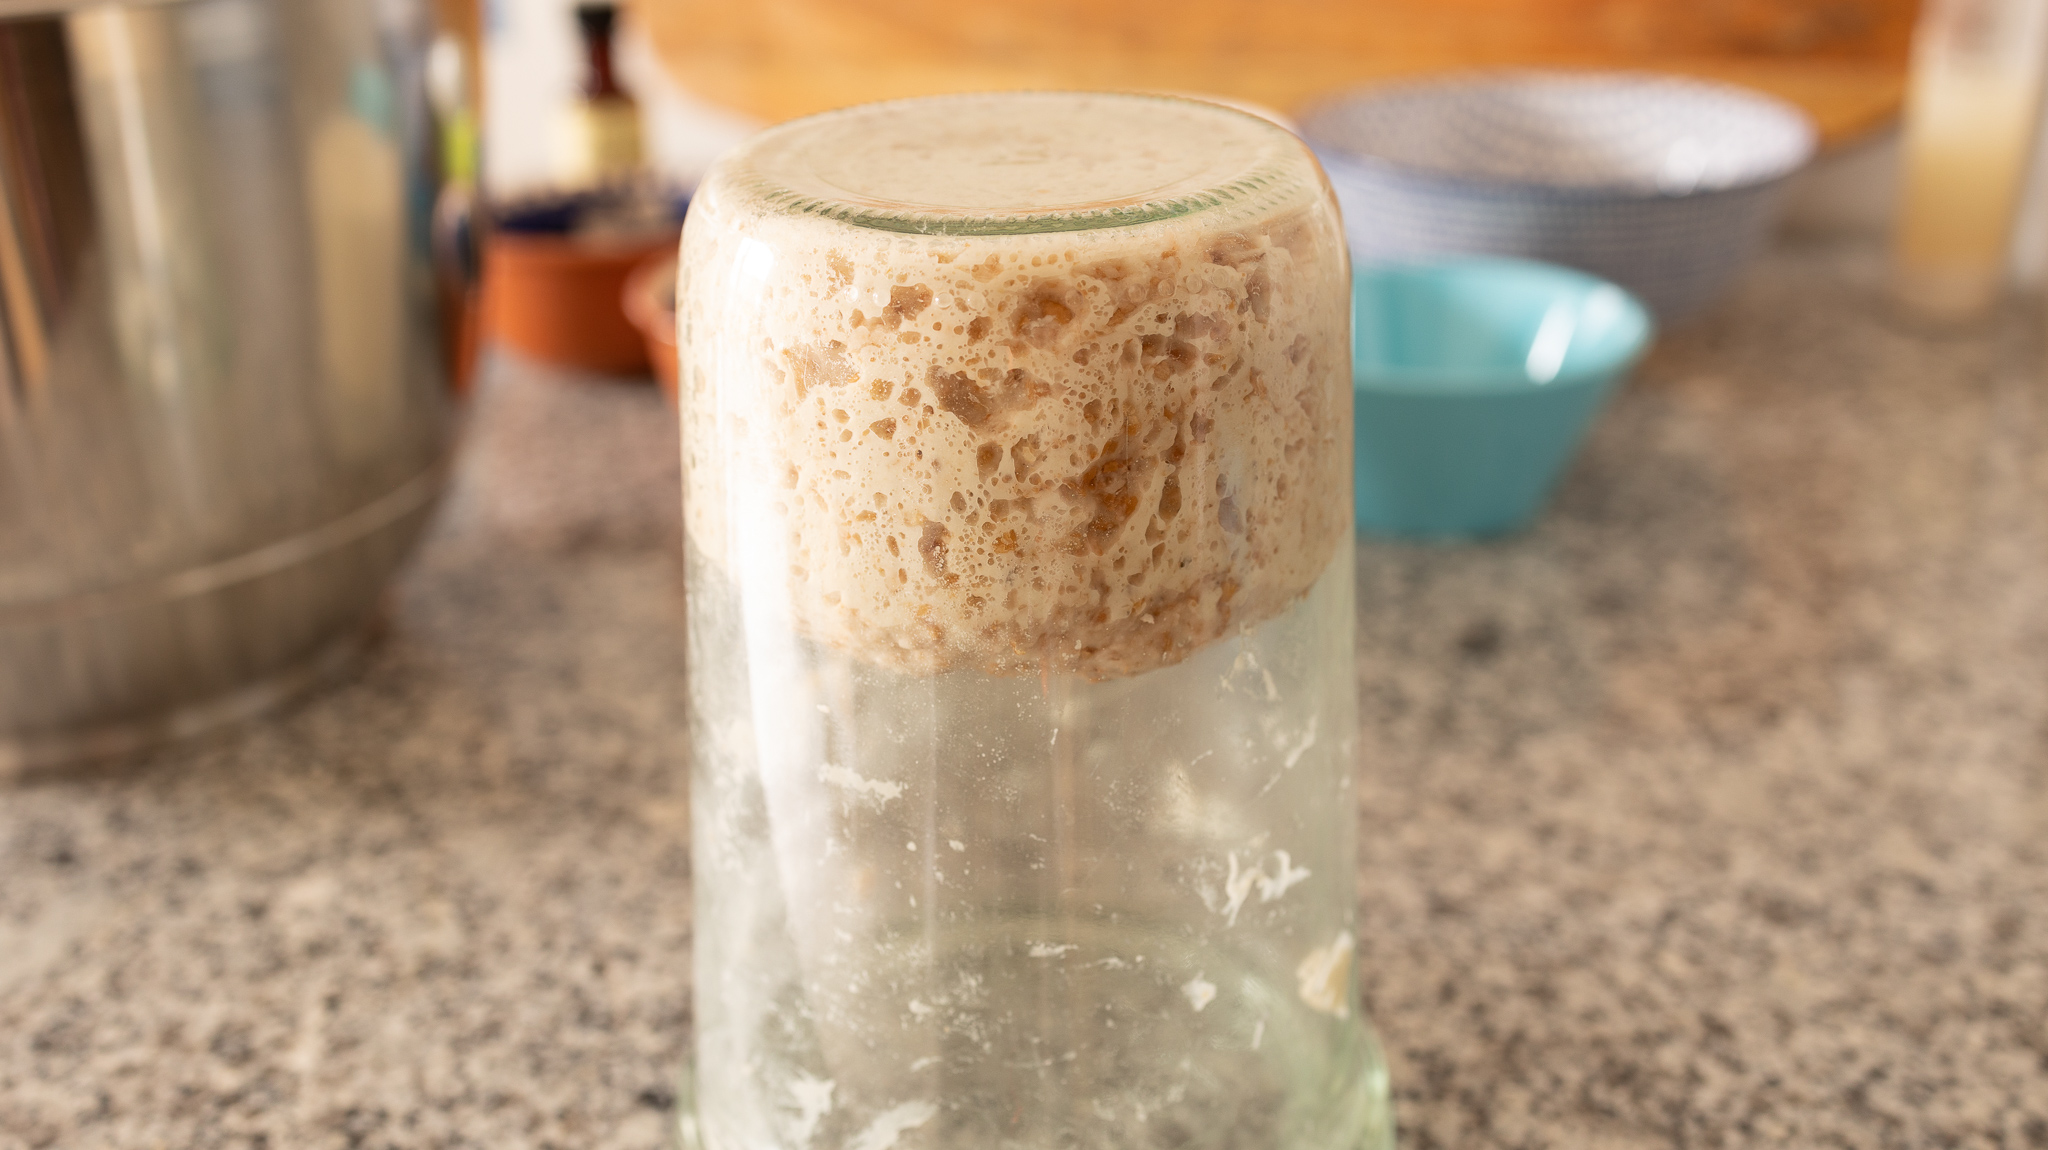
\includegraphics[width=\textwidth]{sourdough-starter-stiff.jpg}
  \caption{A stiff sourdough starter that I~used to make a Stollen dough for Christmas. Note
  the bubbles on the edge of the container. The dough does not fall out of the
jar.}%
  \label{fig:stiff-sourdough-starter}
\end{figure}

The stiff starter is the driest of all the starters. It has a hydration of
around 50 to 60 percent. So for 100 grams of flour you are using around 50 to
60 grams of water. If you can't mix flour and water because the
mixture is too dry you need to increase the water quantity. This is often
the case when using whole wheat/rye flour to make your starter. The
more bran your flour contains, the more water your flour can absorb. The stiff
starter should have a comparable consistency to pasta or pizza dough. When
mixing the starter there should be no chunks of flour left. Test placing
the starter on your kitchen counter. When lifting it should slightly stick
to your counter's surface. This test indicates that you hydrated the flour sufficiently.
When the mixture is too dry, the fermentation speed is greatly reduced and
the starter will seem inactive. The starter should be much drier
than a regular starter, but also not too dry. Refer to figure~\ref{fig:stiff-starter-dry-check}
for a visual example of the starter's required hydration level. 

\begin{figure}[!htb]
  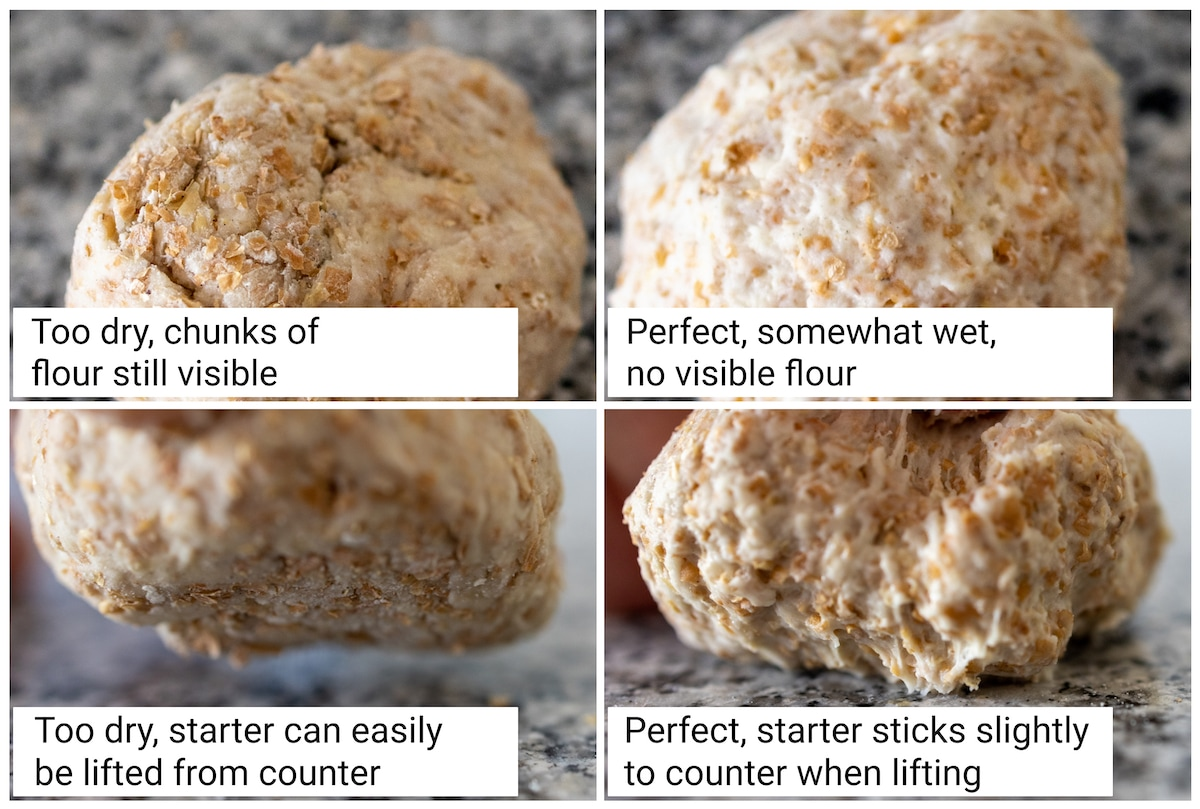
\includegraphics[width=\textwidth]{stiff-starter-dry-check.jpg}
  \caption{An image showing you a stiff starter that is too dry and one that is perfectly hydrated.
  The starter shouldn't contain chunks of flour and slightly stick to your counter top. The
  starter in the picture is made with whole wheat flour.}%
  \label{fig:stiff-starter-dry-check}
\end{figure}

\begin{figure}[!htb]
\begin{center}
  \begin{tikzpicture}[node distance = 3cm, auto]
  \node [start] (init) {Take your regular or liquid starter};
  \node [block, right of=init] (feed_new_ratio) {Mix \qty{10}{\gram} existing starter, \qty{50}{\gram} flour and \qty{25}{\gram} water};
  \node [decision, right of=feed_new_ratio, node distance=3.5cm] (too_dry) {Starter very dry, hard to mix?};
  \node [block, right of=too_dry, node distance=4cm] (add_water) {Add more water};
  \node [block, below of=add_water, node distance=2cm] (next_day) {Wait\\ \qty{24}{\hour}};
  \node [decision, below of=too_dry, node distance=3.5cm] (repeated_3_times) {Stiff starter fed 3 times overall?};
  \node [block, below of=feed_new_ratio, node distance=3.5cm] (feed_again) {Feed again using 1:5:2.5 ratio};
  \node [decision, below of=repeated_3_times, node distance=3.5cm] (ready_signs) {Size increase and sour smell?};
  \node [block, below of=next_day, node distance=2cm] (last_feed) {Feed one last time};
  \node [success, below of=last_feed, node distance=3cm] (bread_dough) {Make bread dough};
  \path [line] (init) -- (feed_new_ratio);
  \path [line] (feed_again) -- (feed_new_ratio);
  \path [line] (next_day) -- (repeated_3_times);
  \path [line] (repeated_3_times) -- node{yes} (ready_signs);
  \path [line] (repeated_3_times) -- node{no} (feed_again);
  \path [line] (ready_signs) -- node{no} (feed_again);
  \path [line] (ready_signs) -- node{yes} (last_feed);
  \path [line] (last_feed) -- node{after \qtyrange{6}{12}{\hour}} (bread_dough);
  \path [line] (feed_new_ratio) -- (too_dry);
  \path [line] (add_water) -- (next_day);
  \path [line] (too_dry) -- node{no} (next_day);
  \path [line] (too_dry) -- node{yes} (add_water);
  \path [line] (ready_signs) -- node{yes} (last_feed);
\end{tikzpicture}

  \caption{The process to convert your regular starter into a stiff starter. The whole
  process takes around 3 days. The longer you maintain your starter at the
  suggested hydration level, the more adapted your microorganisms become. The
  stiff starter boosts the yeast activity of your sourdough starter.
  The guide uses a 50 percent hydration level for the starter. If the dough is too stiff
  consider increasing this to 60 percent.}%
  \label{fig:stiff-starter-conversion}
\end{center}
\end{figure}

In the stiffer environment the yeast thrives more. This means you will have
more \ch{CO2} production and less acid production. In my tests this is a game
changer especially if you are using weaker gluten flours. The wheat flours in
my home country of Germany tend to be lower in gluten. For wheat to build gluten, warm conditions
are preferred~\cite{gluten+development+temperatures}. When following recipes
from other bakers, I~could never achieve similar results. When following
timings my doughs would
simply collapse and become super sticky. Only when I~started to buy more
expensive wheat flour did my results start to change. As not everyone can afford
these special baking flours and due to their limited availability, I~stumbled upon the
stiff sourdough starter. I~made several tests where I~used the same amount of
starter and flour. I~only changed the hydration between all the starters.
I~would then proceed and place a balloon on top of each of the jars. The stiff
starter jar was clearly inflated the most. The regular starter
followed in second place. The liquid starter finished in third place with far less \ch{CO2}
production.

\begin{figure}[!htb]
  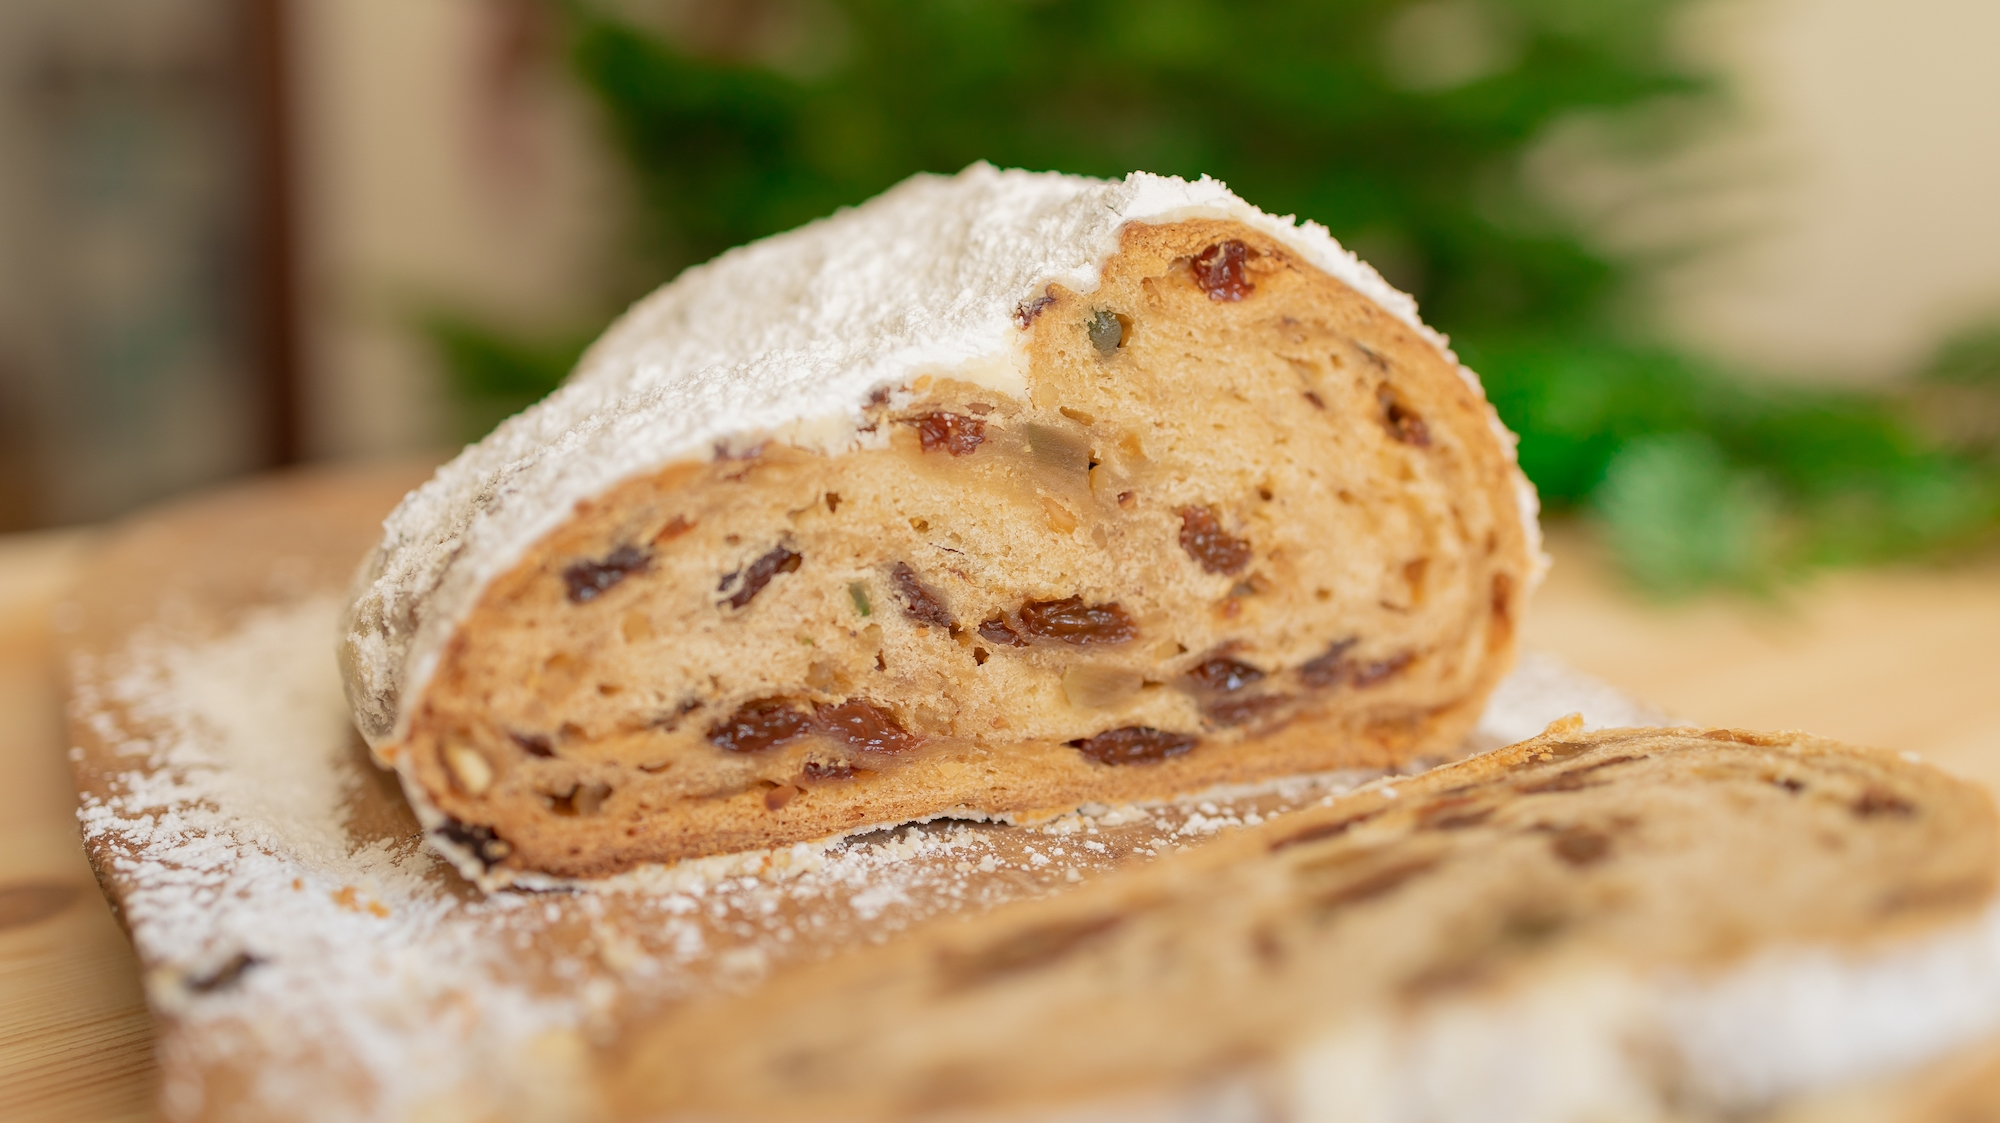
\includegraphics[width=\textwidth]{stollen}
  \caption{A German Christmas stollen made with a stiff starter instead of
  yeast.}%
  \label{fig:stollen}
\end{figure}

I~then proceeded and bought a cheap low cake flour in my nearby supermarket.
This flour before had caused me massive headaches before. I~made a sourdough bread
exactly how I~would normally do. I~had to reduce the hydration a bit as a low
gluten flour does not soak up as much water. Then I~replaced the starter with
the stiff starter. The dough felt amazing and was suddenly able to withstand a
much longer fermentation period. The bread had great oven spring and tasted
very mild. I~am still yet to find a proper explanation why the yeast part of
the dough is more active. Maybe it is not. It could also be that the bacteria
is inhibited by the lack of water.

When making the stiff sourdough starter, start by using around 50 percent
water. If you are using a whole wheat flour, or a strong flour consider going
up to 60 percent. All the ingredients should mix together very well. There
should be no crumbly flour left. This is a common mistake I~have seen when
people tried to make the stiff starter. Yes it should be dry, but not to a
point where it is a brick of cement. If you have ever made a pasta dough, this
dough should feel exactly the same.

To evaluate whether your stiff starter is ready, look for a dome. Also look for
pockets of air on the sides of your container. Use your nose to smell the
starter. It should have a mild smell. It also tends to smell much more
alcoholic than the other starters.

When using a stiff starter, use around 1 to 20 percent depending on the ripeness of
your starter. In summer I~typically use around 10 percent and in winter
around 20 percent. This way you can also control the fermentation speed.
Mixing the starter can be a little bit annoying as it hardly homogenizes with
the rest of the dough. In this case you can try to dissolve the starter in the
water you are about to use for your dough. This will make mixing a lot easier.


\section{Lievito madre or pasta madre}

The lievito madre, also known as pasta madre, belongs to the same category as
the stiff sourdough starter. After conducting hours of research, I~could not
find a difference between pasta madre and lievito madre. Both terms seem to be
used interchangeably in literature.

In many recipes this starter is made directly
from dried or fresh fruits. You can also make a starter from leaves from your
garden. As described before, the wild yeast and bacteria consume the glucose
from the plants' leaves. All the options work. When making a starter directly
from dried fruits, you sometimes lack the bacterial part of the fermentation.
The acidity is very important in order to clean your starter from possible
pathogens. If you decide to make your starter from fruits, make sure it also
acidifies properly when making a dough. A tool such as a pH meter can be of
optimal help. Generally, the lower the pH, the higher the acidity. The acidity
should be below 4.2 to know that your starter produces sufficient acidity.

Some bakers cleanse the lievito madre in a bath of water. This is supposed to
remove excess acidity. In my own experiments I~have not been able to confirm
this methodology. The acidity remains the same. The only reason this could
make sense is if you also tried to boost anaerobic microorganisms. However, then the
starter would need to remain in this environment for quite some time and not just
a few hours.

Baking with sourdough is simple. It's just flour and water. When seeing a recipe
from an experienced baker you wonder, Wait, that's it? There is nothing more
to it? I~feel that this might be the reason why some bakers have such complicated
feeding procedures. They resort to several feedings per day at a certain given ratio.
This makes the baker feel a little more elitist. Of course over time as
more and more people follow this procedure, it becomes a self fulfilling prophecy.
The more experienced you become, the higher the chances are that a bogus starter
feeding guide will reward you with beautiful results. The reason however is
not in the starter routine. The reason is that you understand the fermentation better
and become better at reading the signs of your dough.

If I~had to choose one starter type I~would go for the stiff starter. In many cases
it will provide you with consistently great results with little effort.
In my experience you can make any yeast-based dough and just replace
the yeast directly with the stiff sourdough starter. You will be able
to achieve even better results with the stiff starter.

Lastly, no matter which starter type you choose, you can control how sour
you want your dough to be. The longer you push the fermentation, the more
acidity is going to be piled up. The only difference is that for a given
volume increase, the stiff starter will produce the least acidity. So for a
volume increase of 100 percent, the liquid starter has produced the most acidity,
followed by the regular starter and then the stiff starter. If you wait long
enough, the stiff starter will have produced the same amount of acidity as the
other starters. But before doing so it will have also produced a lot more \ch{CO2}. If
you like the sour flavor, you have to push your fermentation longer. This also
means you either need to bake in a loaf pan or have a very strong gluten flour
that is able to withstand long fermentation times.
